\chapter{Results and evaluation} \label{chap:results}
\section{Table of all results}
e
\section{Iteration 1 results}
As mentioned in \autoref{ssec:iteration1layers}, various combinations of LSTM layers and Dense layers were tested,
each with various sizes. The results of all the models can be seen in \autoref{fig:iteration1_train_accuracy}
and \autoref{fig:iteration1_all_accuracy}.\\
The results of the best model can be seen in \autoref{fig:iteration1_best_accuracy}

\subsection{Accuracies of all tests}
In the charts below, each line represents a combination of different layer types and sizes of the Dense and LSTM layers of the chart.
For both the training and validation accuracy charts, each line has a corresponding line in the loss charts with the same colour.
There are 16 lines in total for this iteration as there were 2 LSTM layer amounts, 2 Dense layer amounts,
2 LSTM layer sizes, and 2 Dense layer sizes in the tests.

\subsubsection{Training accuracies and losses}
\begin{figure}[ht]
    \centering
    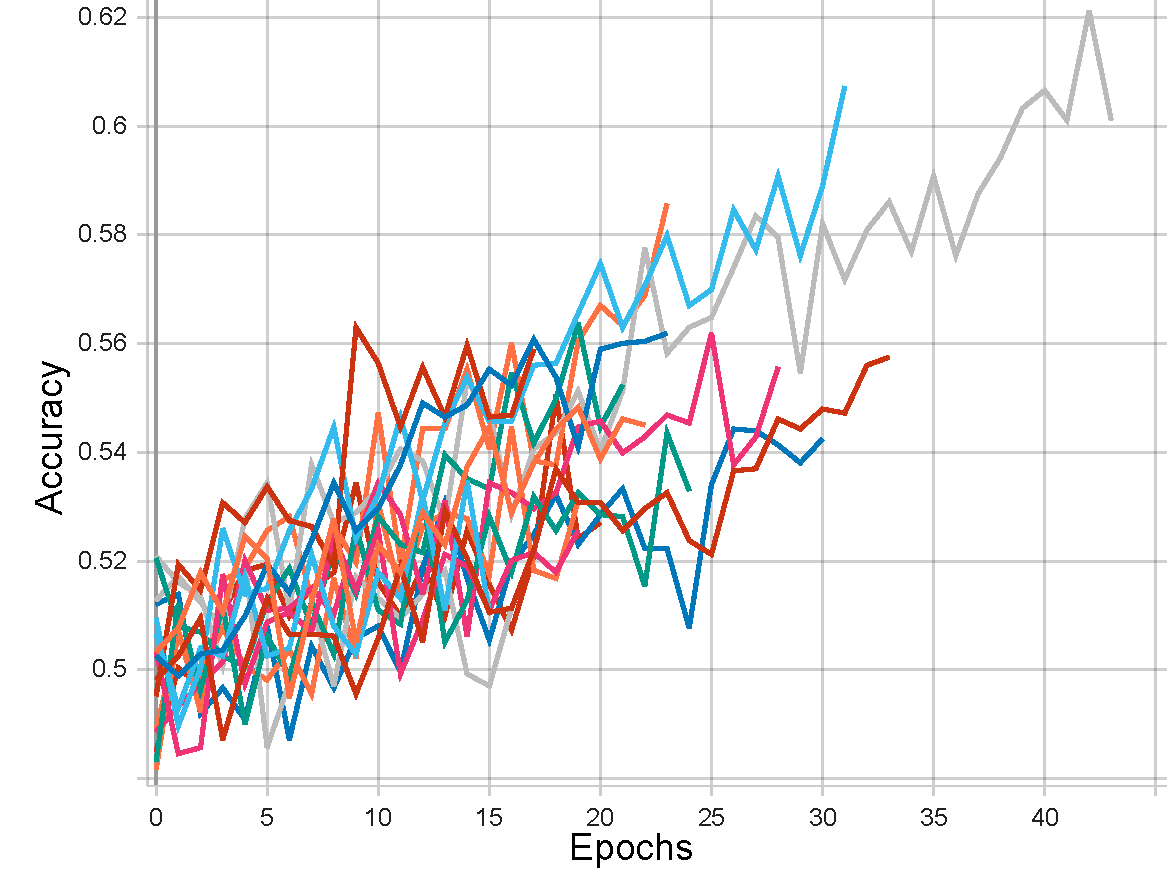
\includegraphics[width=0.95\columnwidth]{figures/results/lstm/lstm_all_acc_t.pdf}
    \caption[Training accuracies for Iteration 1]{Figure of all training accuracies of the combinations of LSTM Layers and Dense Layers in Iteration 1}
    \label{fig:iteration1_train_accuracy}
\end{figure}
\FloatBarrier
\begin{figure}[ht]
    \centering
    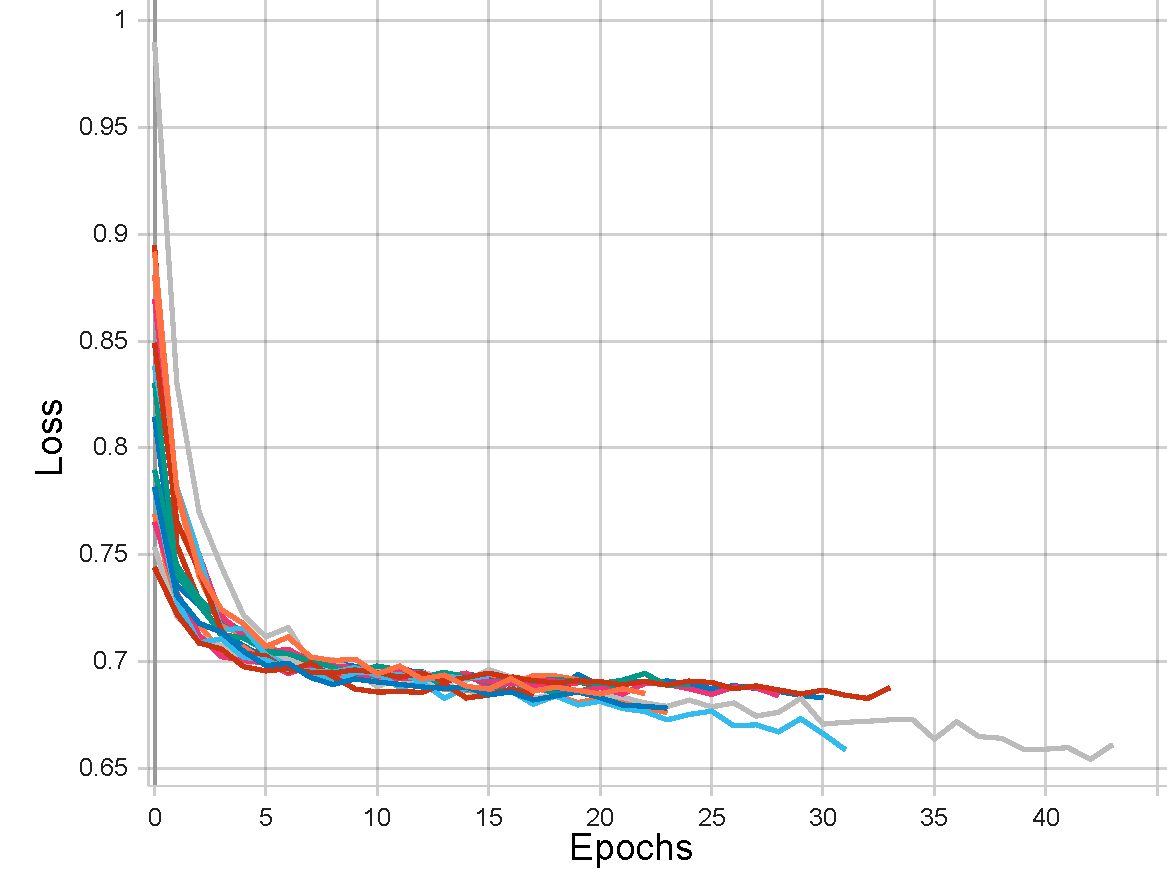
\includegraphics[width=0.95\columnwidth]{figures/results/lstm/lstm_all_loss_t.pdf}
    \caption[Training losses for Iteration 1]{Figure of all training losses of the combinations of LSTM Layers and Dense Layers in Iteration 1}
    \label{fig:iteration1_train_loss}
\end{figure}
\FloatBarrier

\subsubsection{Validation accuracies and losses}
\begin{figure}[ht]
    \centering
    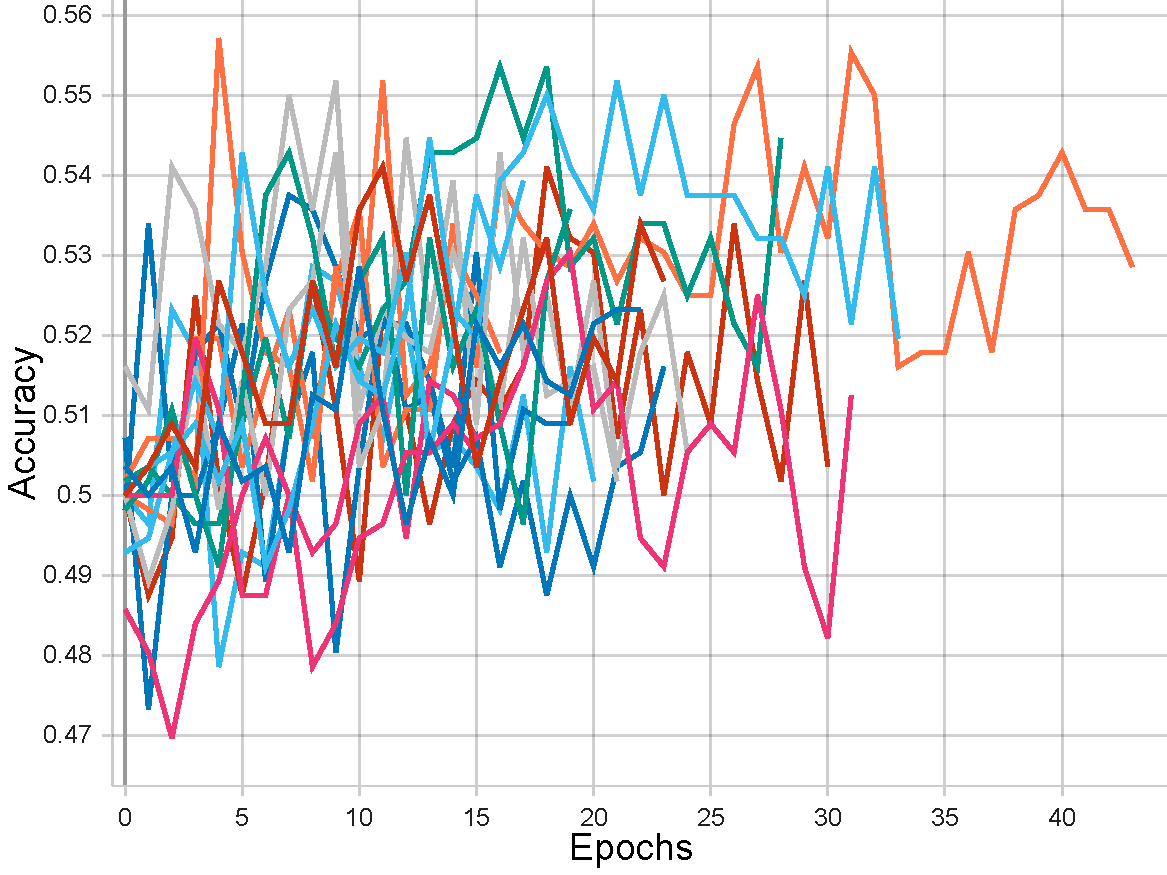
\includegraphics[width=0.95\columnwidth]{figures/results/lstm/lstm_all_acc.pdf}
    \caption[Validation accuracies for Iteration 1]{Figure of all validation accuracies of the combinations of LSTM Layers and Dense Layers in Iteration 1}
    \label{fig:iteration1_all_accuracy}
\end{figure}
\FloatBarrier
\begin{figure}[ht]
    \centering
    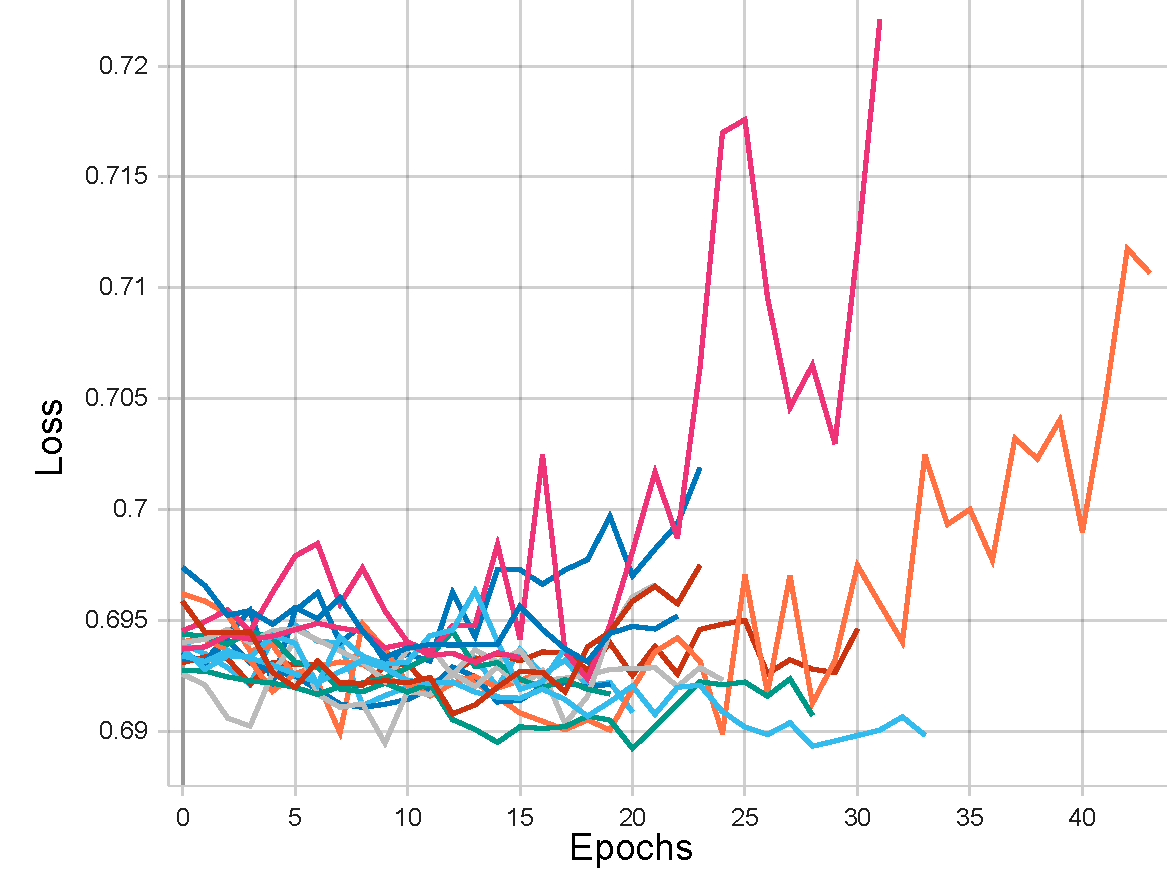
\includegraphics[width=0.95\columnwidth]{figures/results/lstm/lstm_all_loss.pdf}
    \caption[Validation losses for Iteration 1]{Figure of all validation losses of the combinations of LSTM Layers and Dense Layers in Iteration 1}
    \label{fig:iteration1_all_loss}
\end{figure}
\FloatBarrier

There are varying degrees of success with different combinations of layers; some do not improve in accuracy and others do.
The validation losses using the sparse categorical loss function as described earlier in \autoref{sec:model_fitting}
were used to help identify which models had the lowest error rate; and as an increasing validation
loss is an indicator of overfitting, it was used to filter models showing overfitting.

\subsection{Accuracies of the best result}
\begin{figure}[ht]
    \centering
    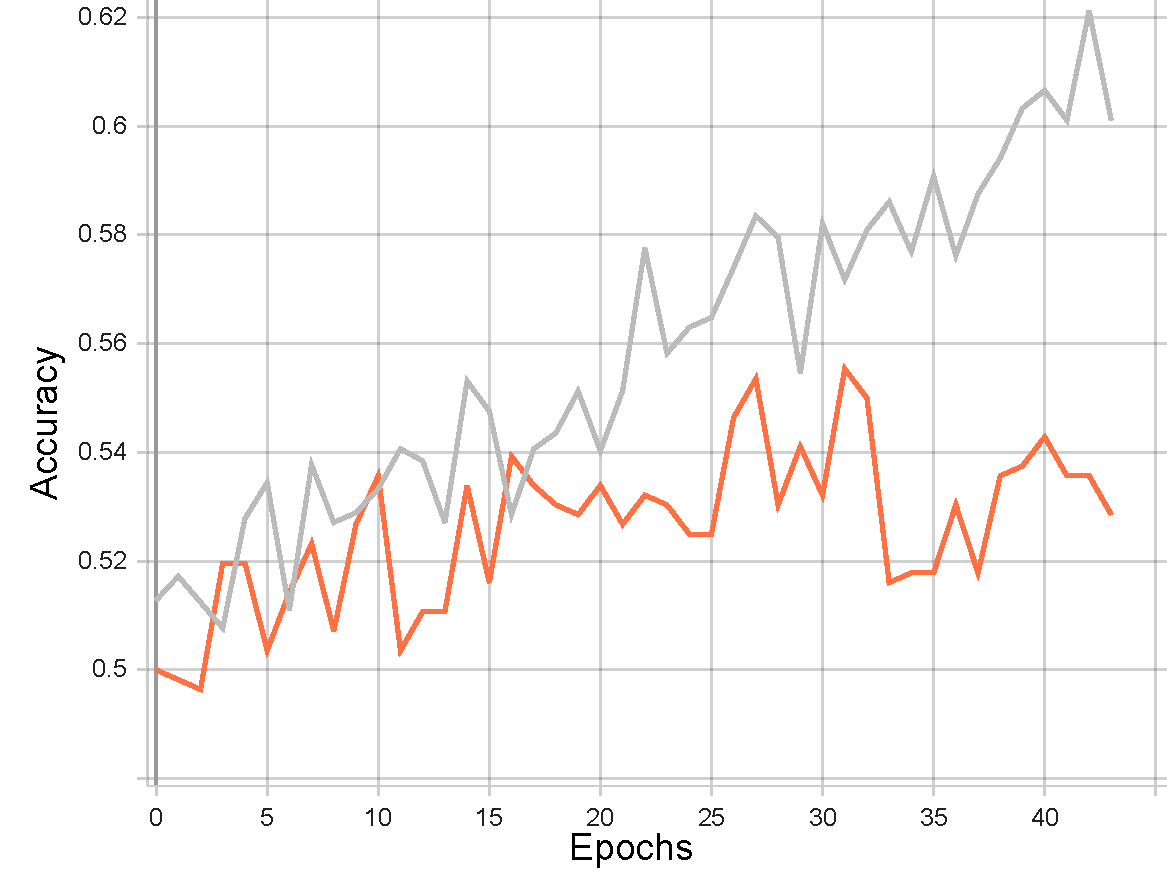
\includegraphics[width=0.95\columnwidth]{figures/results/lstm/lstm_2L64-2D32_acc.pdf}
    \caption[Best accuracy for Iteration 1]{Figure of the best accuracy of the combinations of LSTM Layers and Dense Layers in Iteration 1}
    \label{fig:iteration1_best_accuracy}
\end{figure}
\FloatBarrier
\begin{figure}[ht]
    \centering
    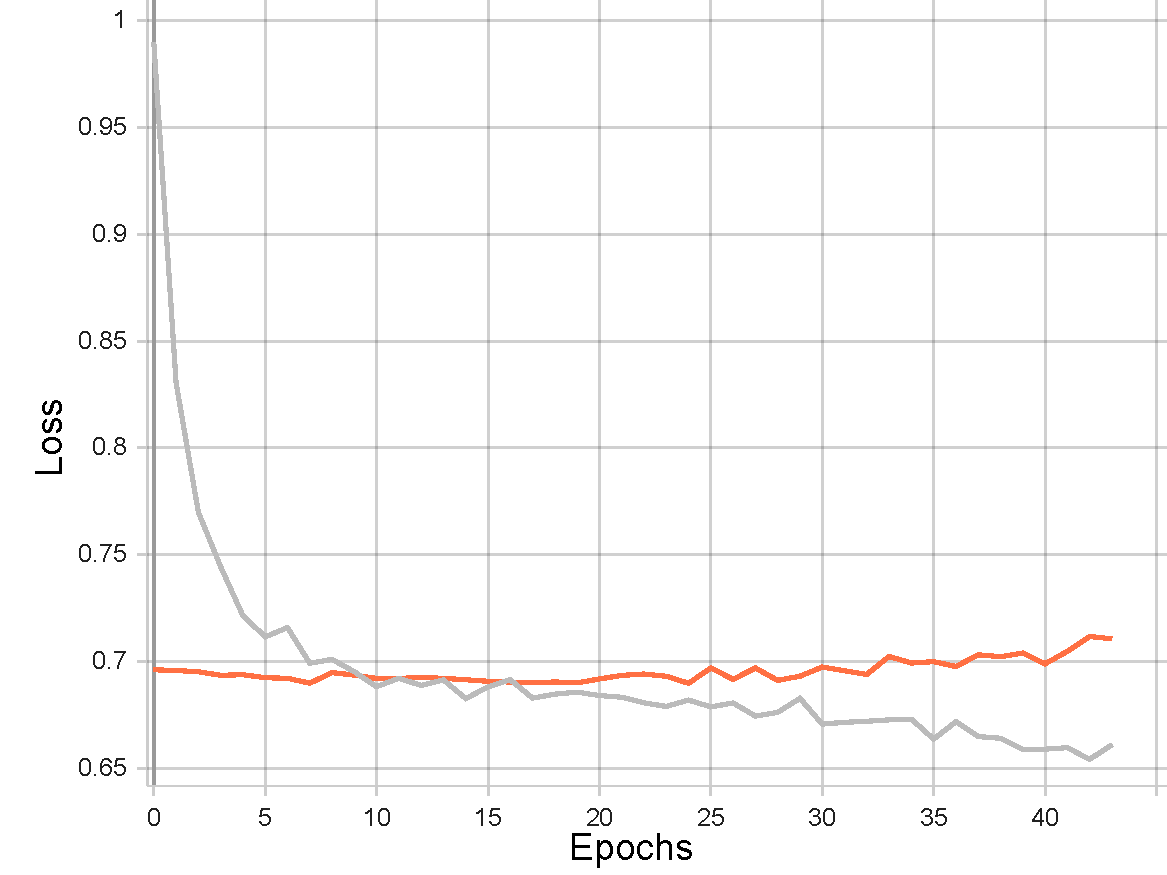
\includegraphics[width=0.95\columnwidth]{figures/results/lstm/lstm_2L64-2D32_loss.pdf}
    \caption[Best loss for Iteration 1]{Figure of the best loss of the combinations of LSTM Layers and Dense Layers in Iteration 1}
    \label{fig:iteration1_best_loss}
\end{figure}
\FloatBarrier
The best model found within this iteration was one with a two LSTM layers of size 64 followed
by the final Dense layer of size 2. The grey line represents the training set and the orange line represents
the validation set. The validation loss shows little overfitting as can be seen in
\autoref{fig:iteration1_best_loss}. At 31 epochs, the validation accuracy reaches its highest value of
55.54\% whilst the training accuracy reached above 57.18\%.
\subsection{Evaluation of iteration 1}
With a validation accuracy above 55\% it suggests that there is improvement above a random choice. It forms a good
basis for testing further AI models, specifically the CNN-LSTM hybrid model.
There are various limitations regarding iteration 1. This iteration does not test various combinations of
input features nor does it test various sequence lengths. Furthermore, there could be another number of layers or
layer sizes that is better suited to the problem, but unfortunately many have not been tested due to time constraints.

\section{Iteration 2 results}
As mentioned in \autoref{ssec:iteration2layers}, various combinations of Conv1D layers and Dense layers were tested,
each with various sizes. The results of all the models can be seen in \autoref{fig:iteration2_train_accuracy}
and \autoref{fig:iteration2_all_accuracy}.\\
The results of the best model can be seen in \autoref{fig:iteration2_best_accuracy}.

\subsection{Accuracies of all tests}
In the charts below, each line represents a combination of different layer types and sizes of the Dense and LSTM layers of the chart.
For both the training and validation accuracy charts, each line has a corresponding line in the loss charts with the same colour.
There are 16 lines in total for this iteration as there were 2 Conv1D layer amounts, 2 Dense layer amounts,
2 Conv1D layer sizes, and 2 Dense layer sizes in the tests.

\subsubsection{Training accuracies and losses}
\begin{figure}[ht]
    \centering
    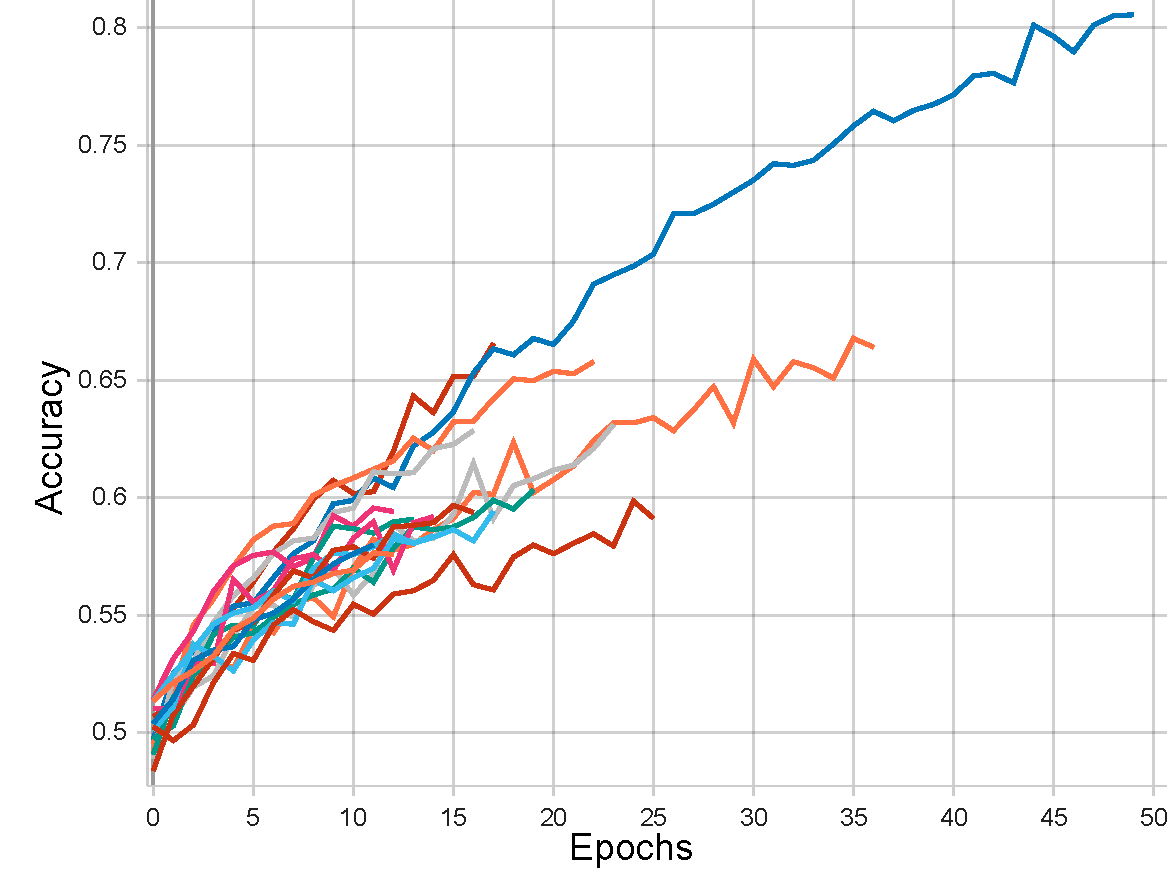
\includegraphics[width=0.95\columnwidth]{figures/results/cnn/cnn_all_acc_t.pdf}
    \caption[Training accuracies for Iteration 2]{Figure of all training accuracies of the combinations of Conv1D Layers and Dense Layers in Iteration 2}
    \label{fig:iteration2_train_accuracy}
\end{figure}
\FloatBarrier
\begin{figure}[ht]
    \centering
    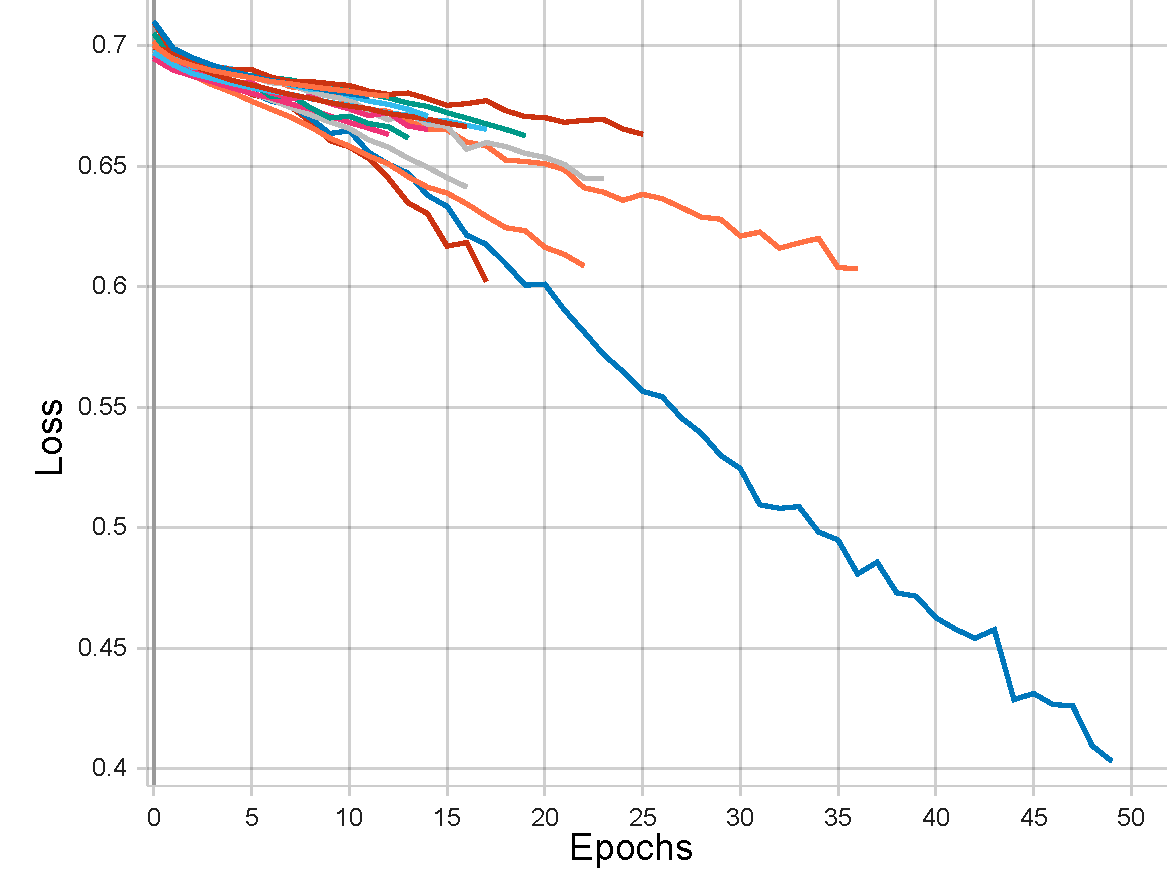
\includegraphics[width=0.95\columnwidth]{figures/results/cnn/cnn_all_loss_t.pdf}
    \caption[Training losses for Iteration 2]{Figure of all training losses of the combinations of Conv1D Layers and Dense Layers in Iteration 2}
    \label{fig:iteration2_train_loss}
\end{figure}
\FloatBarrier

\subsubsection{Validation accuracies and losses}
\begin{figure}[ht]
    \centering
    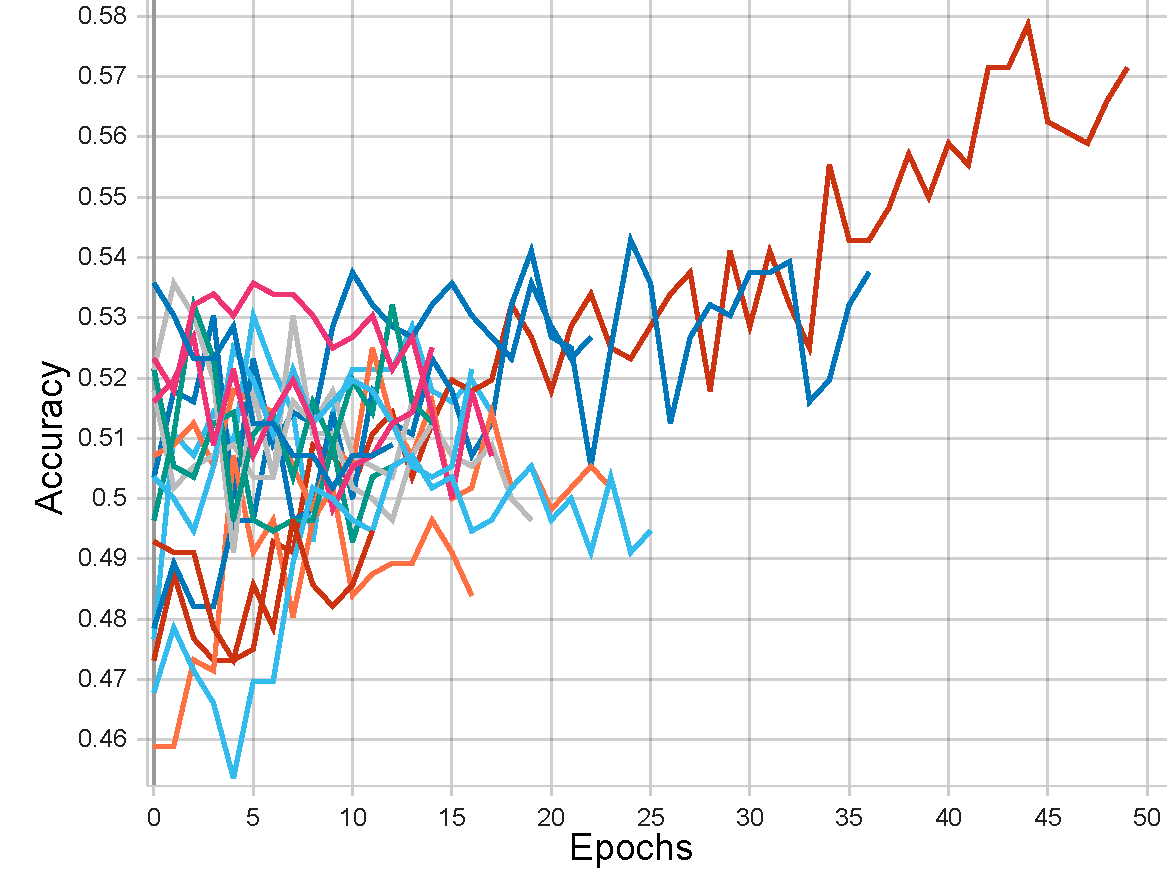
\includegraphics[width=0.95\columnwidth]{figures/results/cnn/cnn_all_acc.pdf}
    \caption[Validation accuracies for Iteration 2]{Figure of all validation accuracies of the combinations of Conv1D Layers and Dense Layers in Iteration 2}
    \label{fig:iteration2_all_accuracy}
\end{figure}
\FloatBarrier
\begin{figure}[ht]
    \centering
    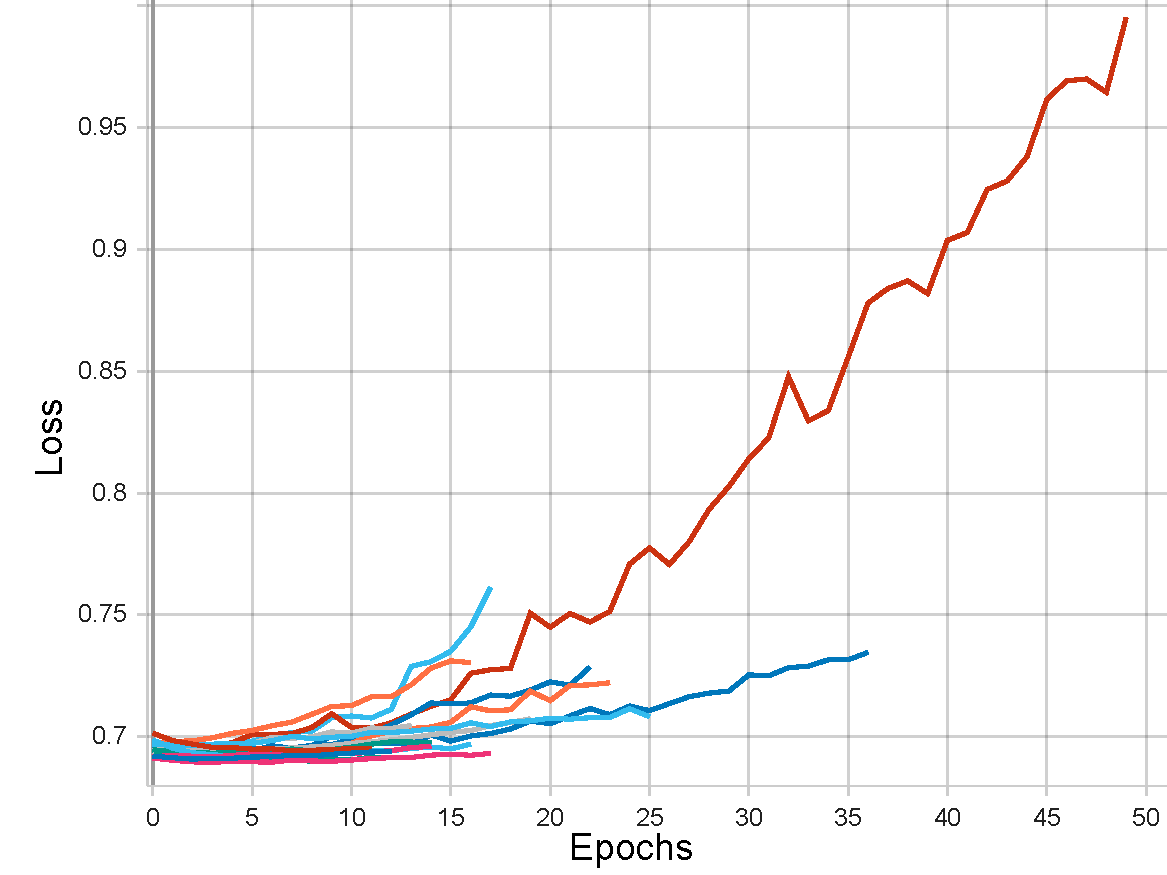
\includegraphics[width=0.95\columnwidth]{figures/results/cnn/cnn_all_loss.pdf}
    \caption[Validation losses for Iteration 2]{Figure of all validation losses of the combinations of Conv1D Layers and Dense Layers in Iteration 2}
    \label{fig:iteration2_all_loss}
\end{figure}
\FloatBarrier

There are varying degrees of success with different combinations of layers; some do not improve in accuracy and others do.
The validation losses using the sparse categorical loss function as described earlier in \autoref{sec:model_fitting}
were used to help identify which models had the lowest error rate; and as an increasing validation
loss is an indicator of overfitting, it was used to filter models showing overfitting.

\subsection{Accuracies of the best result}
\begin{figure}[ht]
    \centering
    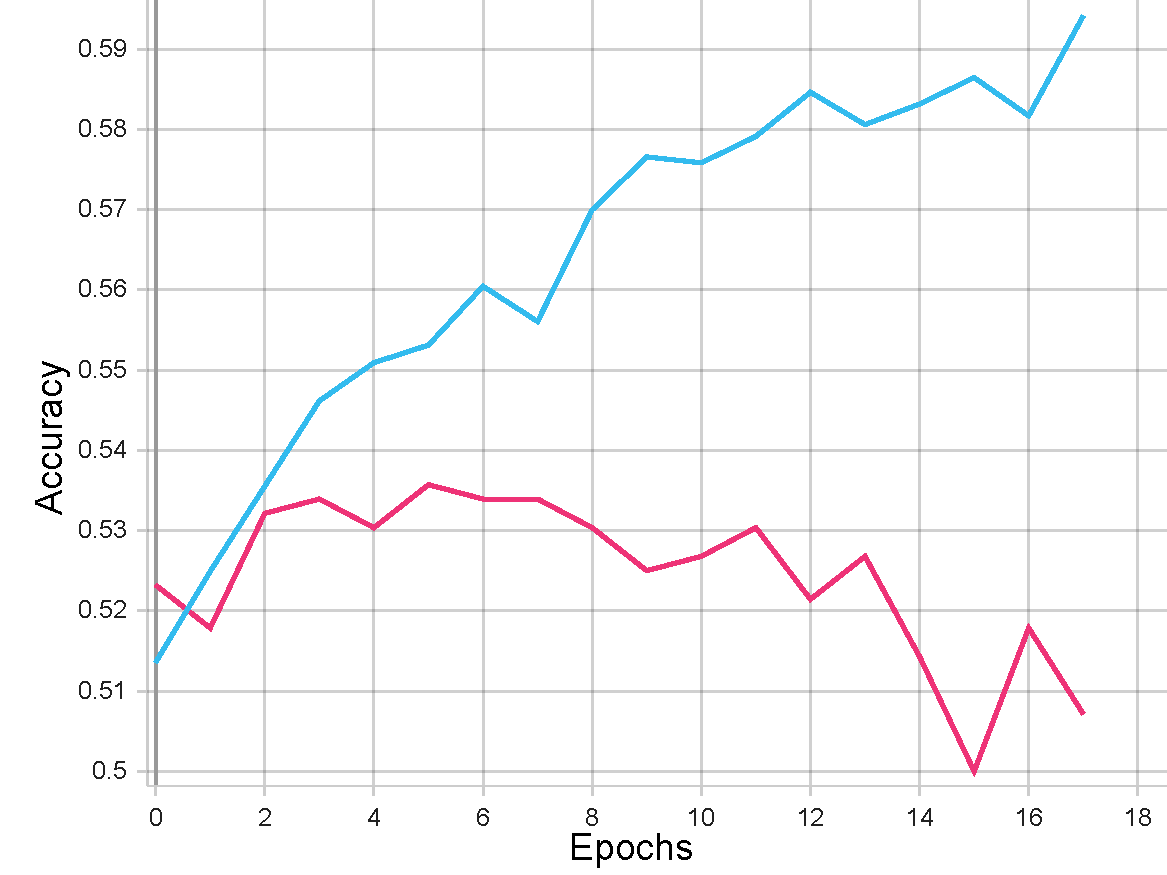
\includegraphics[width=0.95\columnwidth]{figures/results/cnn/cnn_1C32-1D64_acc.pdf}
    \caption[Best accuracy for Iteration 2]{Figure of the best accuracy of the combinations of Conv1D Layers and Dense Layers in Iteration 2}
    \label{fig:iteration2_best_accuracy}
\end{figure}
\FloatBarrier
\begin{figure}[ht]
    \centering
    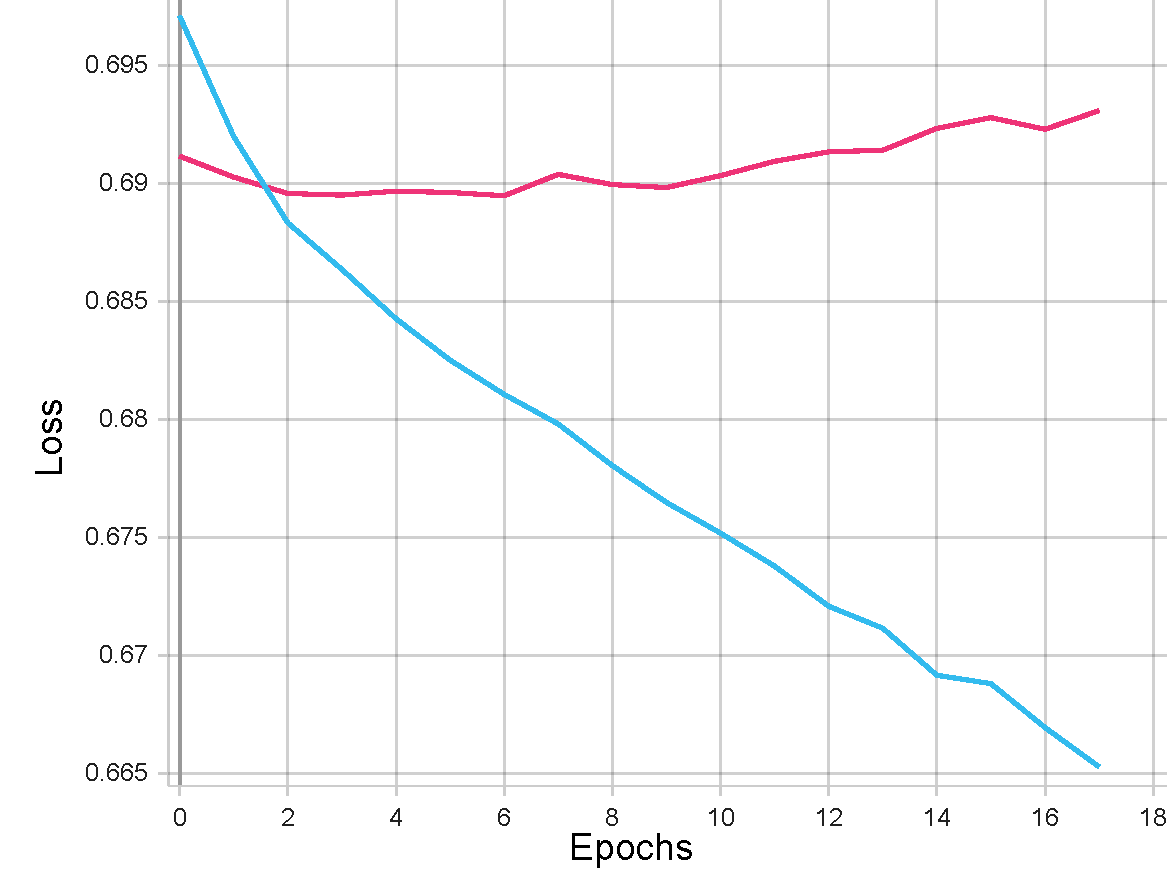
\includegraphics[width=0.95\columnwidth]{figures/results/cnn/cnn_1C32-1D64_loss.pdf}
    \caption[Best loss for Iteration 2]{Figure of the best loss of the combinations of Conv1D Layers and Dense Layers in Iteration 2}
    \label{fig:iteration2_best_loss}
\end{figure}
\FloatBarrier
The best model found within this iteration was one with a one CNN layer of size 32 followed
by the final Dense layer of size 2. The blue line represents the training set and the pink line represents
the validation set. The validation loss shows little overfitting as can be seen in
\autoref{fig:iteration2_best_loss}. At 5 epochs, the validation accuracy reaches its highest value of
53.57\% whilst the training accuracy reached above 55.31\%.
\subsection{Evaluation of iteration 2}
With a validation accuracy above 53\% it suggests that there is only minimal improvement above a random choice. It forms a good
basis for testing further AI models, specifically the CNN-LSTM hybrid model.
There are various limitations regarding iteration 2. This iteration does not test various combinations of
input features nor does it test various sequence lengths. Furthermore, there could be another number of layers or
layer sizes that is better suited to the problem, but unfortunately many have not been tested due to time constraints.

\section{Iteration 3 results}
As mentioned in \autoref{ssec:iteration3layers}, various combinations of Conv1D layers, LSTM layers and Dense layers were tested,
each with various sizes. The results of all the models can be seen in \autoref{fig:iteration3_train_accuracy}
and \autoref{fig:iteration3_all_accuracy}.\\
The results of the best model can be seen in \autoref{fig:iteration3_best_accuracy}.

\subsection{Accuracies of all tests}
In the charts below, each line represents a combination of different layer types and sizes of the Conv1D, LSTM and Dense layers.
For both the training and validation accuracy charts, each line has a corresponding line in the loss charts with the same colour.
There are 64 lines in total for this iteration as there were 2 Conv1D layer amounts, 2 LSTM layer amounts, 2 Dense layer amounts,
as well as 2 Conv1D layer sizes, 2 LSTM layer sizes and 2 Dense layer sizes in the tests.

\subsubsection{Training accuracies and losses}
\begin{figure}[ht]
    \centering
    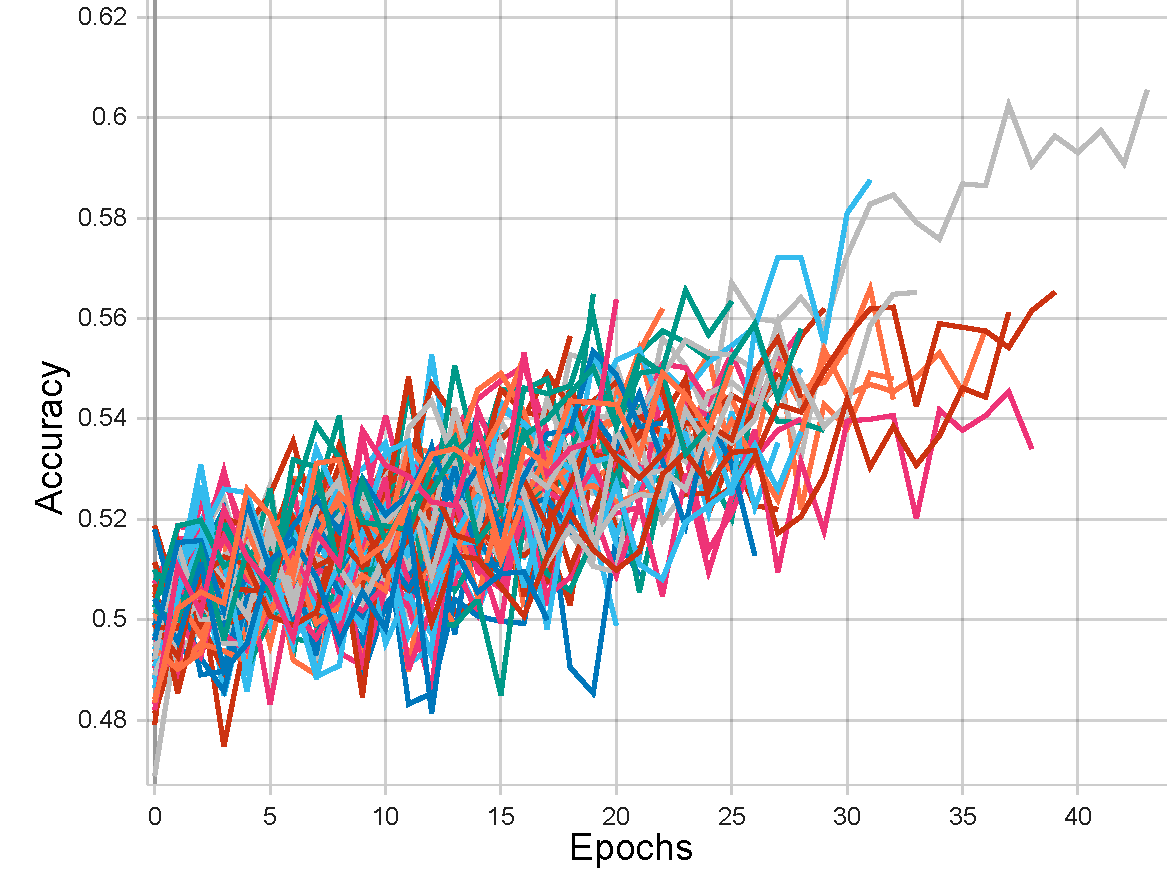
\includegraphics[width=0.95\columnwidth]{figures/results/cnnlstm/cnnlstm_all_acc_t.pdf}
    \caption[Training accuracies for Iteration 3]{Figure of all training accuracies of the combinations of Conv1D, LSTM and Dense Layers in Iteration 3}
    \label{fig:iteration3_train_accuracy}
\end{figure}
\FloatBarrier
\begin{figure}[ht]
    \centering
    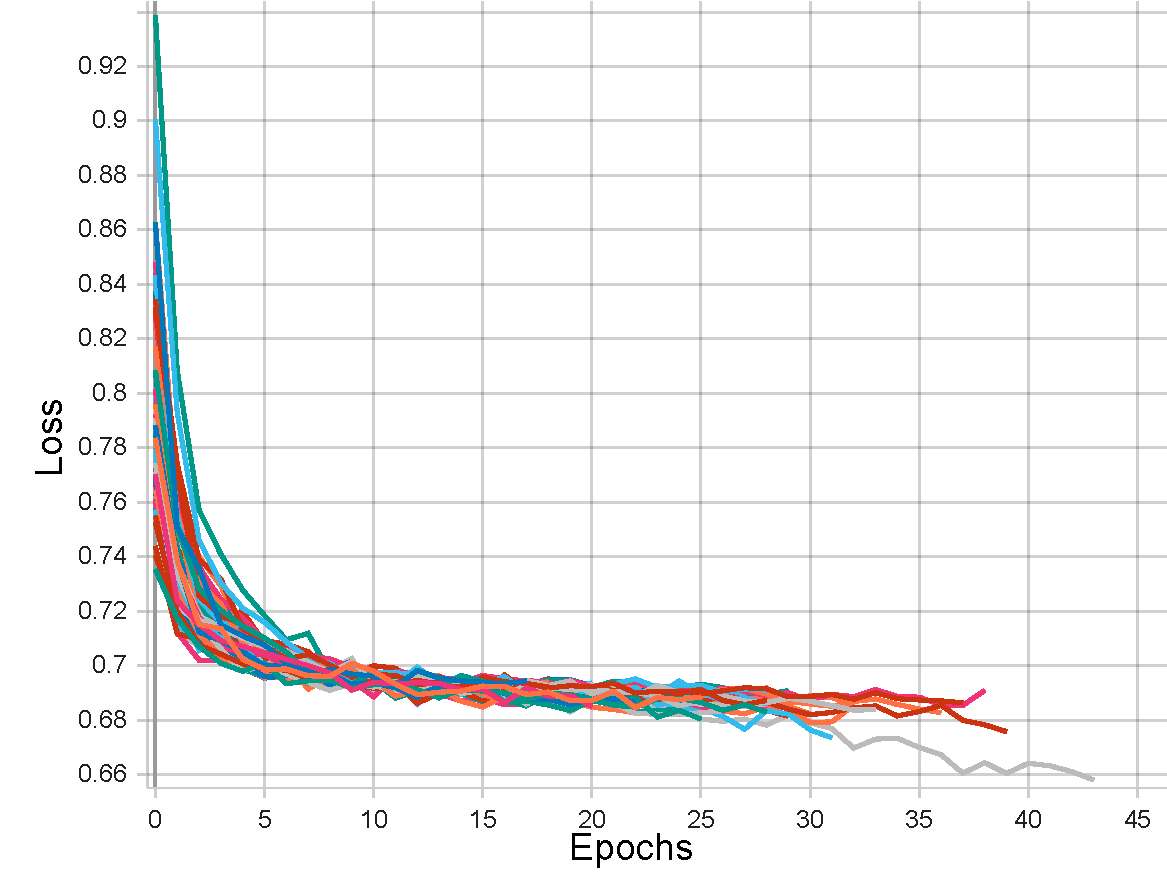
\includegraphics[width=0.95\columnwidth]{figures/results/cnnlstm/cnnlstm_all_loss_t.pdf}
    \caption[Training losses for Iteration 3]{Figure of all training losses of the combinations of Conv1D, LSTM and Dense Layers in Iteration 3}
    \label{fig:iteration3_train_loss}
\end{figure}
\FloatBarrier

\subsubsection{Validation accuracies and losses}
\begin{figure}[ht]
    \centering
    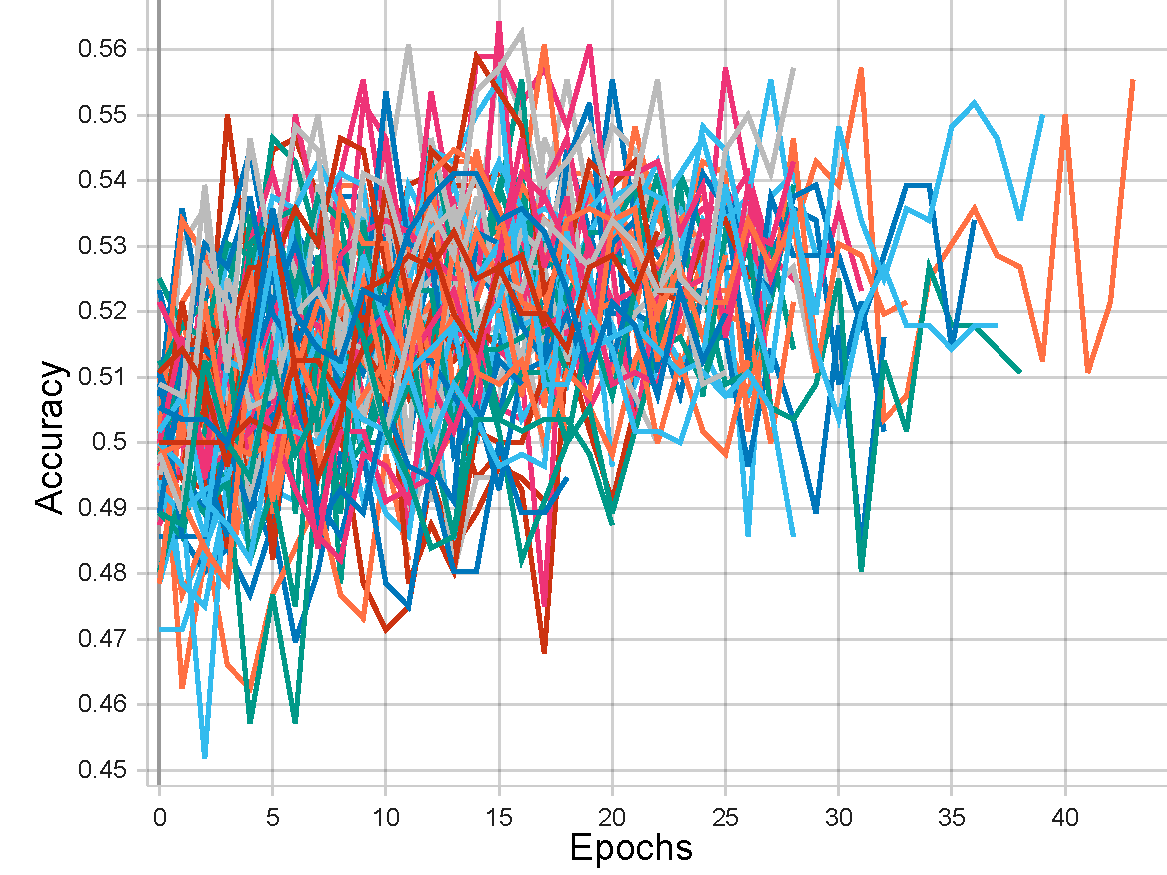
\includegraphics[width=0.95\columnwidth]{figures/results/cnnlstm/cnnlstm_all_acc.pdf}
    \caption[Validation accuracies for Iteration 3]{Figure of all validation accuracies of the combinations of Conv1D, LSTM and Dense Layers in Iteration 3}
    \label{fig:iteration3_all_accuracy}
\end{figure}
\FloatBarrier
\begin{figure}[ht]
    \centering
    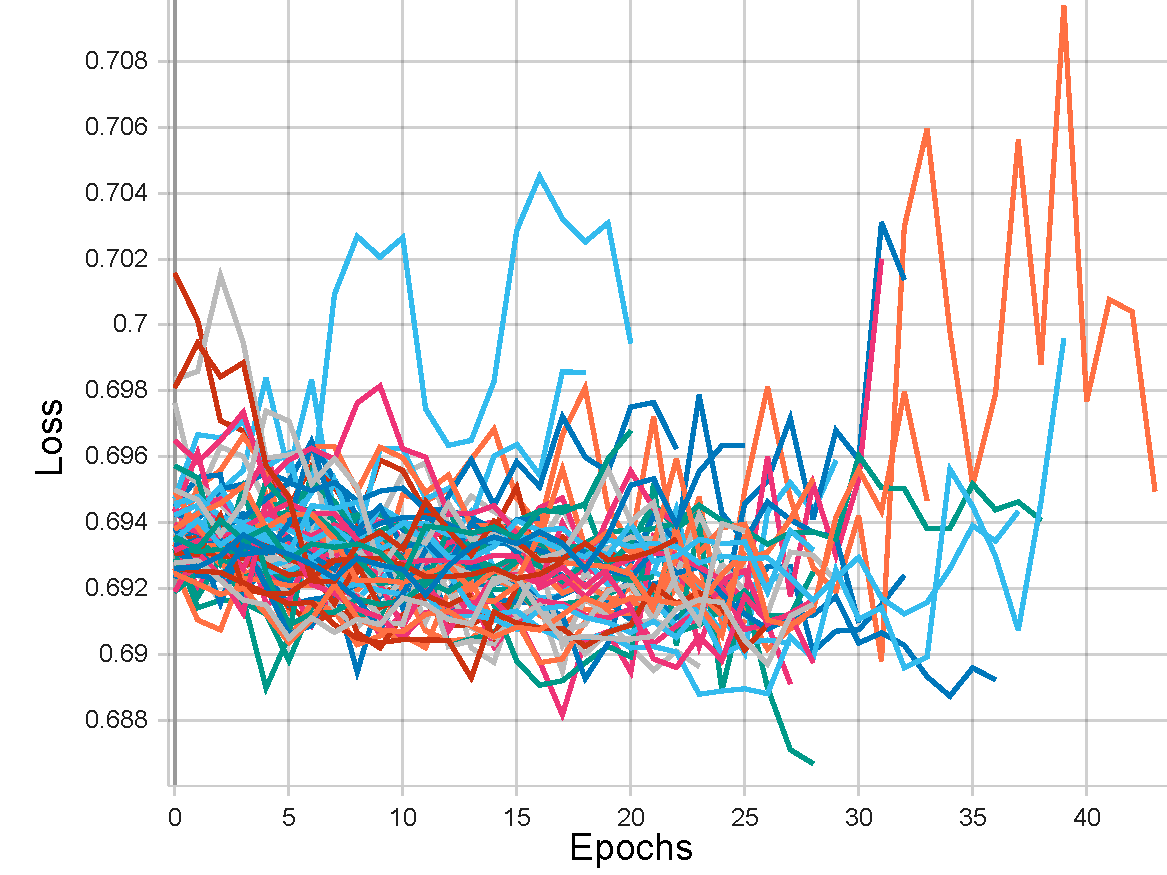
\includegraphics[width=0.95\columnwidth]{figures/results/cnnlstm/cnnlstm_all_loss.pdf}
    \caption[Validation losses for Iteration 3]{Figure of all validation losses of the combinations of Conv1D, LSTM and Dense Layers in Iteration 3}
    \label{fig:iteration3_all_loss}
\end{figure}
\FloatBarrier

There are varying degrees of success with different combinations of layers; some do not improve in accuracy and others do.
The validation losses using the sparse categorical loss function as described earlier in \autoref{sec:model_fitting}
were used to help identify which models had the lowest error rate; and as an increasing validation
loss is an indicator of overfitting, it was used to filter models showing overfitting.

\subsection{Accuracies of the best result}
\begin{figure}[ht]
    \centering
    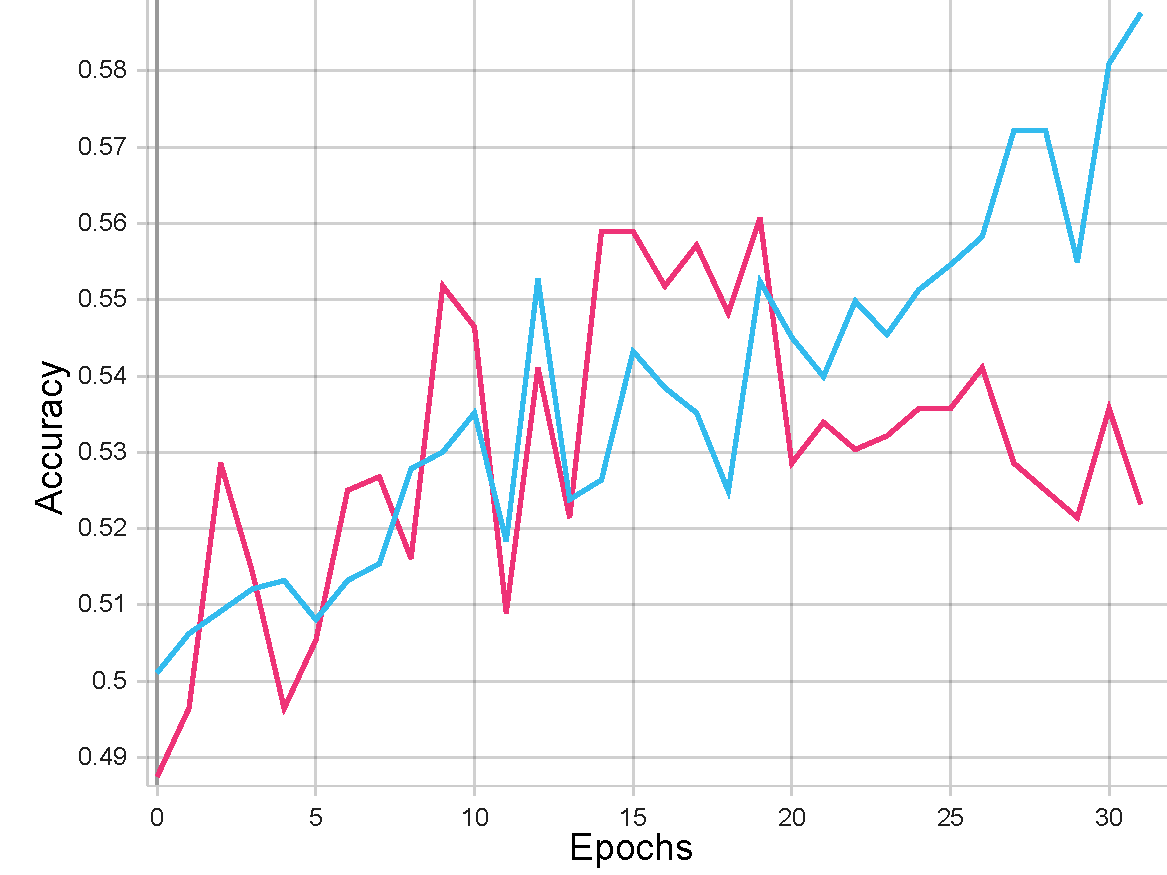
\includegraphics[width=0.95\columnwidth]{figures/results/cnnlstm/cnnlstm_2C32-1L16-2D64_acc.pdf}
    \caption[Best accuracy for Iteration 3]{Figure of the best accuracy of the combinations of Conv1D, LSTM and Dense Layers in Iteration 3}
    \label{fig:iteration3_best_accuracy}
\end{figure}
\FloatBarrier
\begin{figure}[ht]
    \centering
    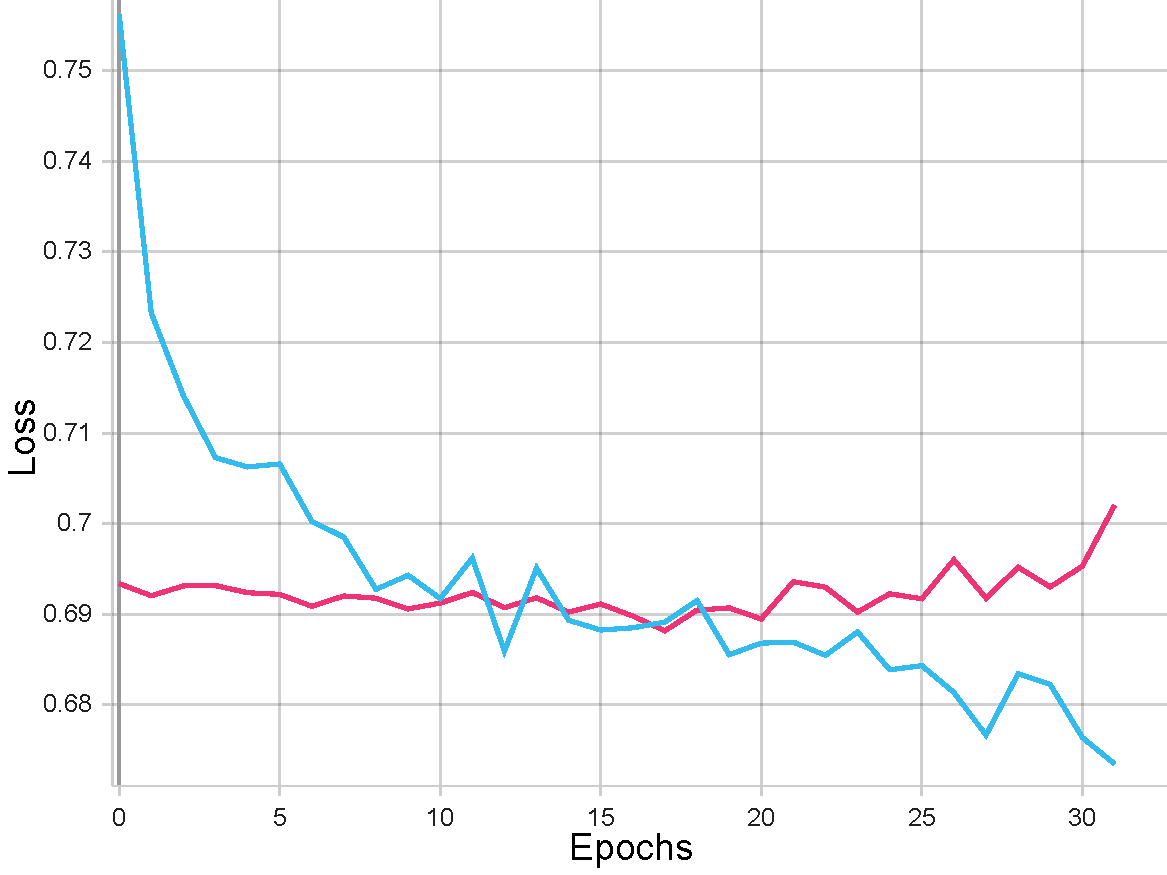
\includegraphics[width=0.95\columnwidth]{figures/results/cnnlstm/cnnlstm_2C32-1L16-2D64_loss.pdf}
    \caption[Best loss for Iteration 3]{Figure of the best loss of the combinations of Conv1D, LSTM and Dense Layers in Iteration 3}
    \label{fig:iteration3_best_loss}
\end{figure}
\FloatBarrier
The best model found within this iteration was one with a two Conv1D layers of size 32 followed by 1 LSTM layer
of size 16, and a Dense layer of size 64 followed by a final Dense layer of size 2.
The blue line represents the training set and the pink line represents
the validation set. The validation loss shows little overfitting as can be seen in
\autoref{fig:iteration3_best_loss}. At 19 epochs, the validation accuracy reaches its highest value of
56.07\% whilst the training accuracy reached 55.24\%. The validation accuracy being somewhat greater than the
training accuracy can be explained by the dropout layers within the model that can affect the results of the training
set but does not affect the validation set.

\subsection{Evaluation of iteration 3}
With a validation accuracy above 56.07\%, it is currently the best model when compared to the previous iterations.
This suggests there is a significant advantage compared to randomly guessing the next trading day's direction.
Furthermore, this aligns with the studies analysed in the literature review. However, this iteration alone cannot be
used to answer the research questions as it does not test different sequence lengths or combinations of input features.
Additionally, there could be a different number of layers or sizes of layers that perform better but unfortunately could
not be tested due to time constraints.

\section{Iteration 4 results}
As mentioned in \autoref{ssec:iteration4_ai_model}, a concatenated model of the best models of the previous 
three iterations were combined in parallel. The results of this model can be seen in
\autoref{fig:iteration4_accuracy}.

\begin{figure}[ht]
    \centering
    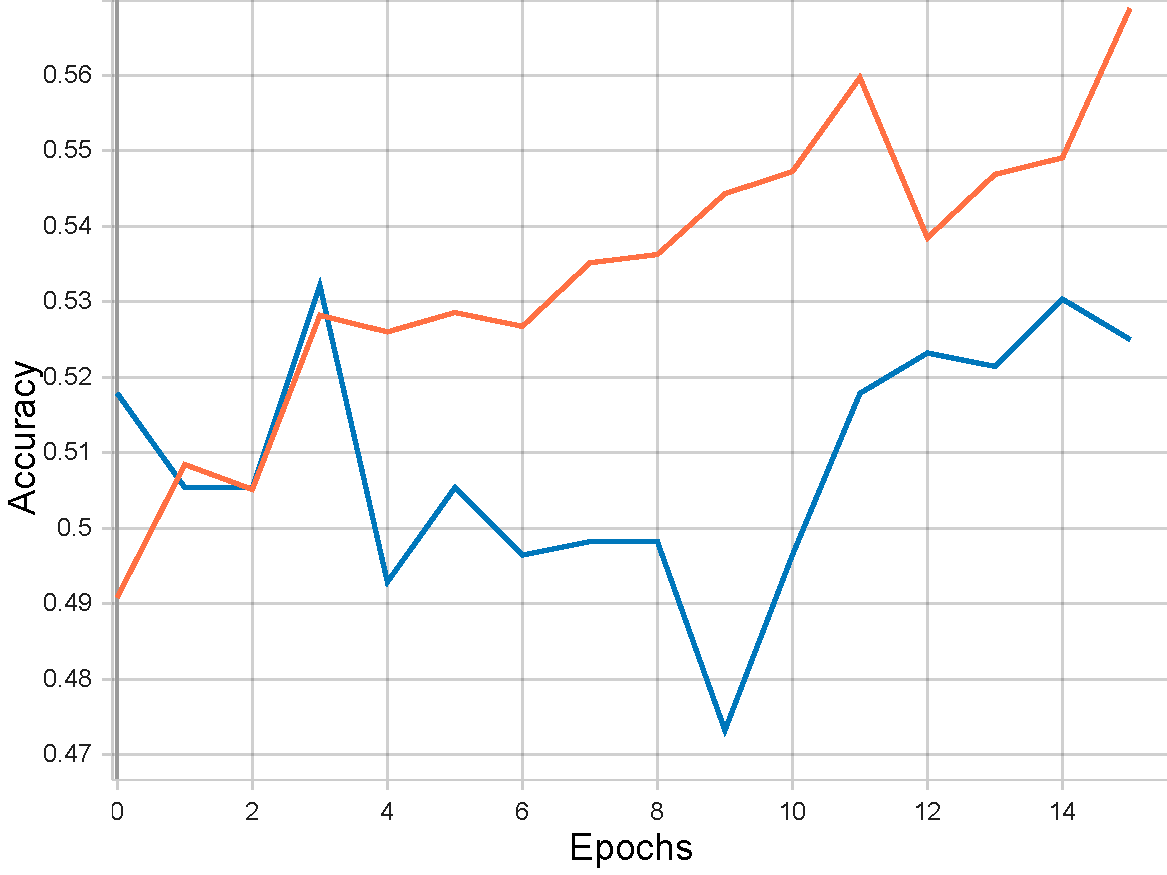
\includegraphics[width=0.95\columnwidth]{figures/results/concat/concat_acc.pdf}
    \caption[Accuracies for Iteration 4]{Figure of all training and validation accuracies in Iteration 4}
    \label{fig:iteration4_accuracy}
\end{figure}
\FloatBarrier
\begin{figure}[ht]
    \centering
    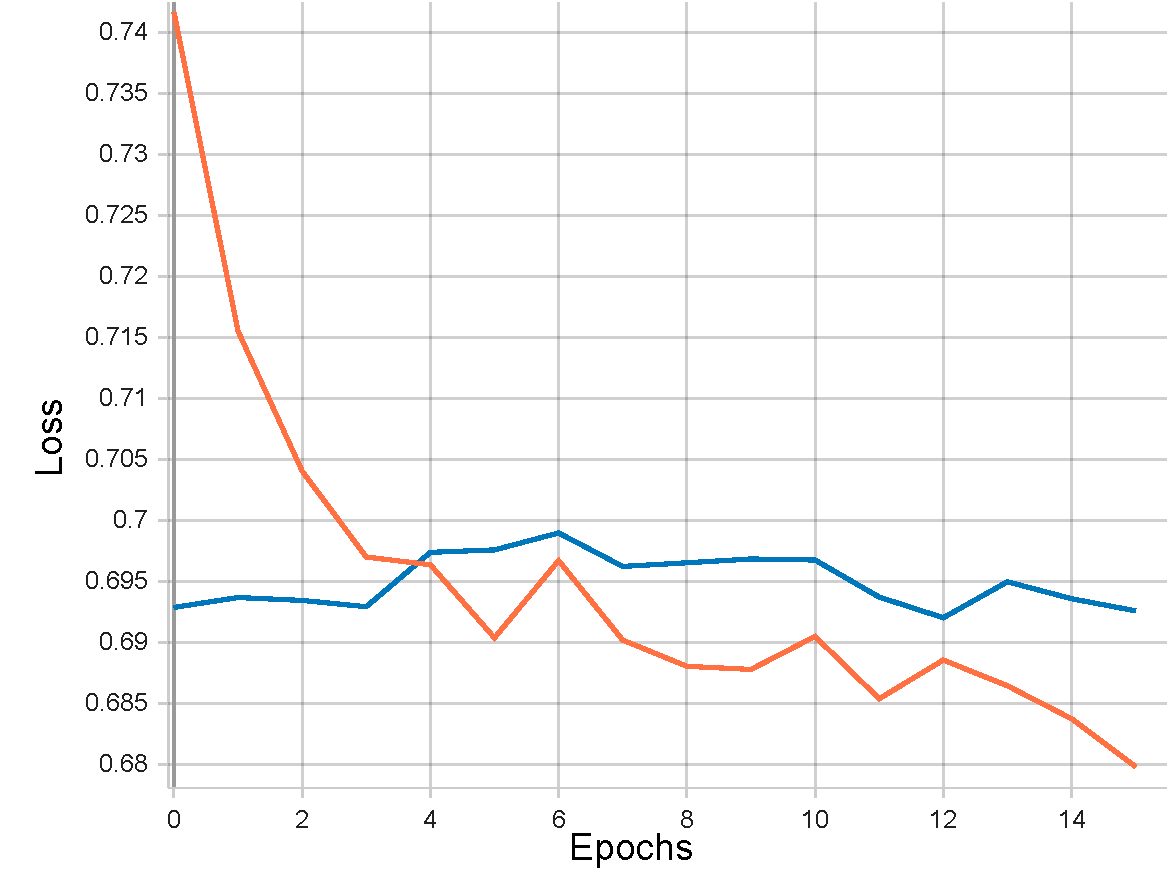
\includegraphics[width=0.95\columnwidth]{figures/results/concat/concat_loss.pdf}
    \caption[Losses for Iteration 4]{Figure of all training and validation losses in Iteration 4}
    \label{fig:iteration4_loss}
\end{figure}
\FloatBarrier

The orange line represents the training set and the blue line represents
the validation set. The validation loss shows little overfitting as can be seen in
\autoref{fig:iteration4_loss} as the loss does not significantly increase. At 3 epochs,
the validation accuracy reaches its highest value of 53.21\% whilst the training accuracy reached 52.82\%. The validation accuracy being somewhat greater than the
training accuracy can be explained by the dropout layers within the model that can affect the results of the training
set but does not affect the validation set.

\subsection{Evaluation of iteration 4}
With a validation accuracy above 53\%, there is only a minimal improvement above a random guess of the direction
of the next trading day. This model was included to test between a sequential hybrid model as seen in Iteration 3
and this parallel hybrid approach. However, this model does not offer any advantage over the CNN-LSTM sequential
model alone; due to this, no further tests will be utilised with this model.

\section{Iteration 5 results}
This iteration primarily used a similar model to that in Iteration 3, however with varied input features
and varied sequence lengths. There are various results that come from this model from identifying the
best amount of historic data to identifying the most important inputs.

\subsection{Accuracies of all tests}

For each of the tests in Iteration 5, the charts contain 15 lines representing the different combinations
of input features as mentioned in \autoref{ssec:iteration5_input_features}. Each line in the accuracy chart
has a corresponding line in the loss chart with the same colour. Each line in the training charts has a 
corresponding line in the validation charts with a different colour.\\
\\
The best values of the validation accuracies of each model at any epoch are shown in
\autoref{ssec:iteration5_best_val_acc}.

\subsubsection{Two days of historic data accuracies and losses}
\textbf{Training accuracies and losses}
\begin{figure}[ht]
    \centering
    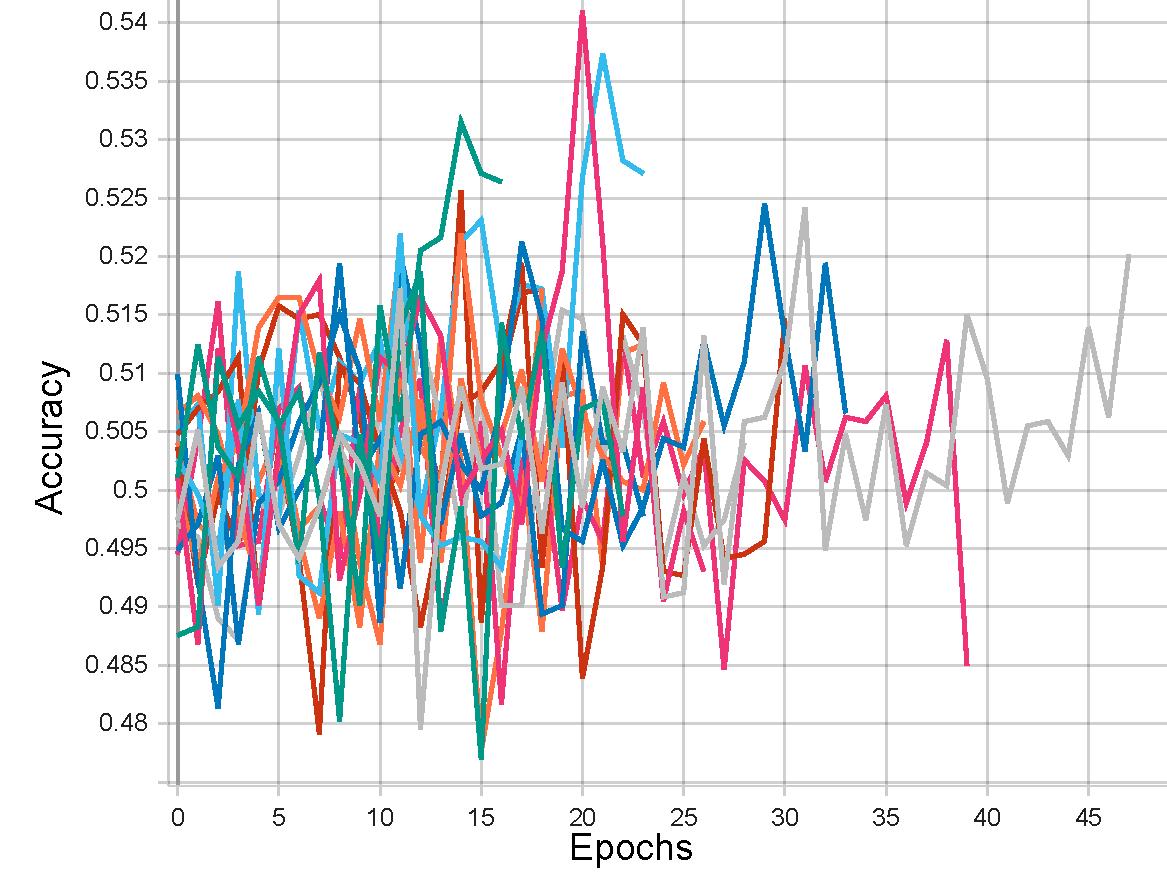
\includegraphics[width=0.575\columnwidth]{figures/results/final/two_days_acc_t.pdf}
    \caption[Training accuracies for Iteration 5 with two days of historic data]{Figure of all training accuracies with two days of historic data in Iteration 5}
    \label{fig:iteration5_two_days_train_accuracy}
\end{figure}
\FloatBarrier
\begin{figure}[ht]
    \centering
    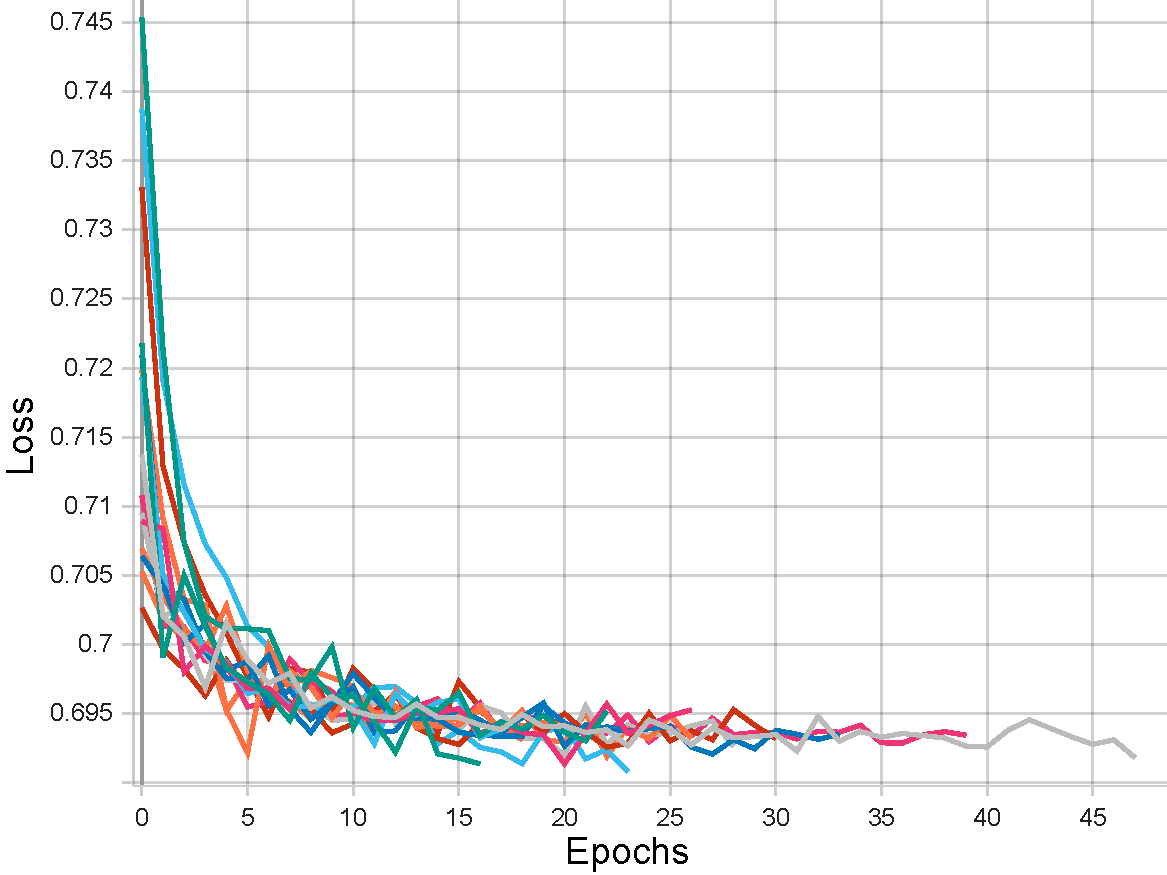
\includegraphics[width=0.575\columnwidth]{figures/results/final/two_days_loss_t.pdf}
    \caption[Training losses for Iteration 5 with two days of historic data]{Figure of all training losses with two days of historic data in Iteration 5}
    \label{fig:iteration5_two_days_train_loss}
\end{figure}
\FloatBarrier

\pagebreak
\textbf{Validation accuracies and losses}
\begin{figure}[ht]
    \centering
    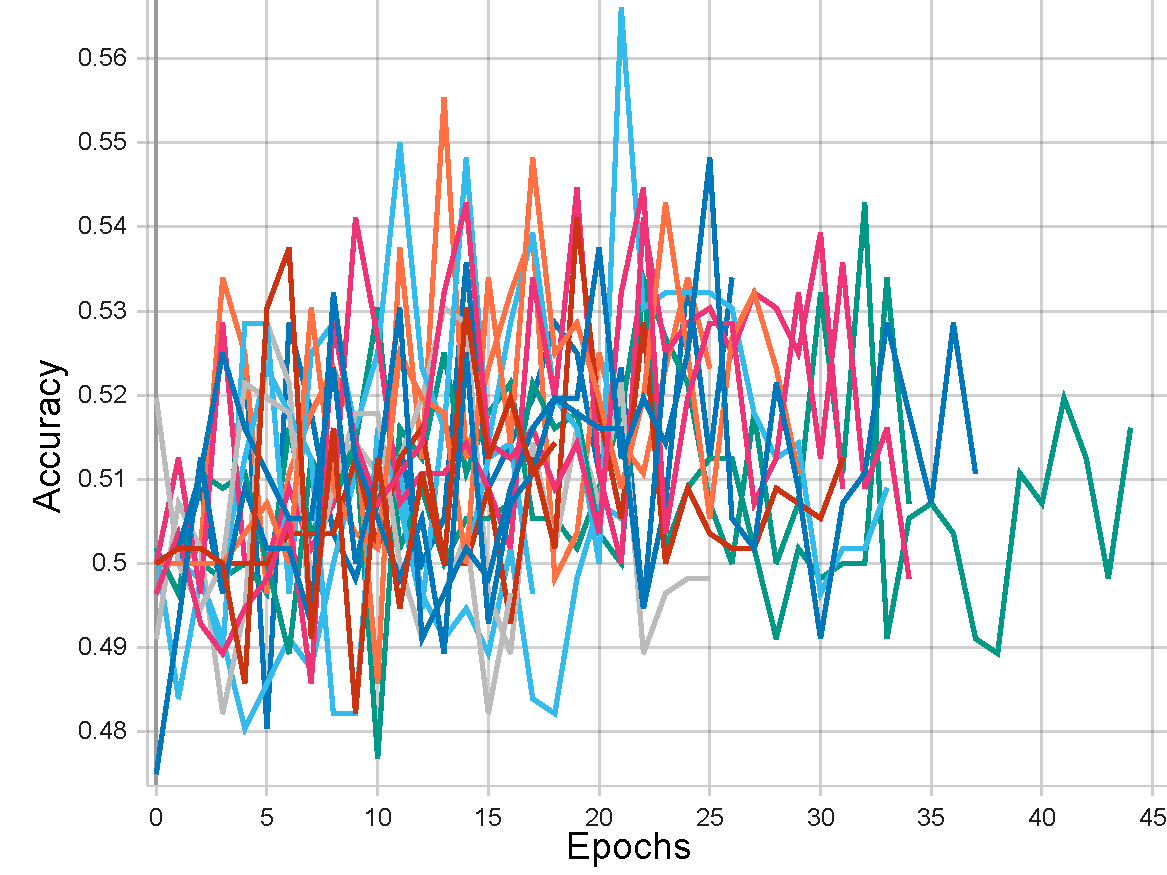
\includegraphics[width=0.575\columnwidth]{figures/results/final/two_days_acc.pdf}
    \caption[Validation accuracies for Iteration 5 with two days of historic data]{Figure of all validation accuracies with two days of historic data in Iteration 5}
    \label{fig:iteration5_two_days_accuracy}
\end{figure}
\FloatBarrier
\begin{figure}[ht]
    \centering
    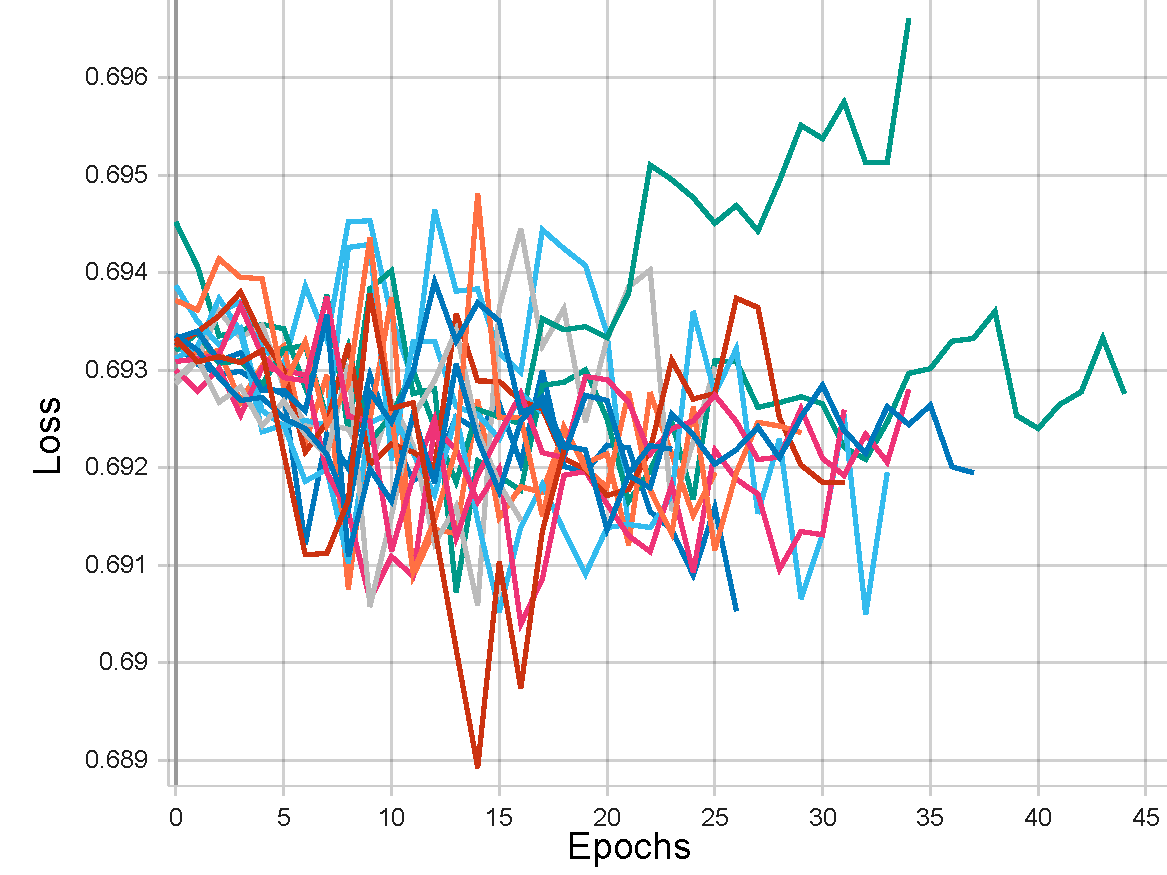
\includegraphics[width=0.575\columnwidth]{figures/results/final/two_days_loss.pdf}
    \caption[Validation losses for Iteration 5 with two days of historic data]{Figure of all validation losses with two days of historic data in Iteration 5}
    \label{fig:iteration5_two_days_loss}
\end{figure}
\FloatBarrier

The greatest validation accuracy for the model with a sequence length of two days was 55.54\% with the dataset using price and volatility data.
While the chart above in \autoref{fig:iteration5_two_days_loss} may look erratic, the loss is actually minimal due to the scale as it only varies
between 0.689 and 0.697. This suggests there is little overfitting as it does not increase significantly.

\pagebreak
\subsubsection{One week of historic data accuracies and losses}
\textbf{Training accuracies and losses}
\begin{figure}[ht]
    \centering
    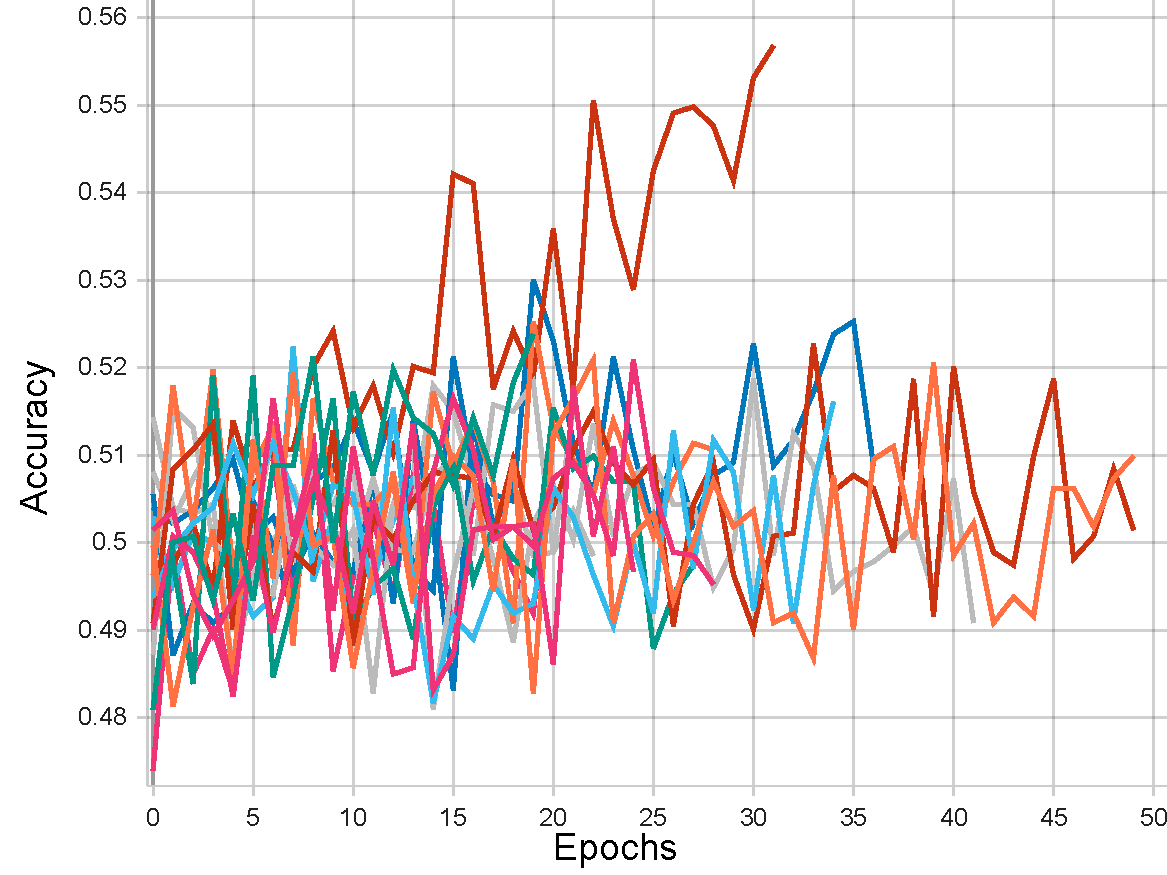
\includegraphics[width=0.575\columnwidth]{figures/results/final/week_acc_t.pdf}
    \caption[Training accuracies for Iteration 5 with one week of historic data]{Figure of all training accuracies with one week of historic data in Iteration 5}
    \label{fig:iteration5_week_train_accuracy}
\end{figure}
\FloatBarrier
\begin{figure}[ht]
    \centering
    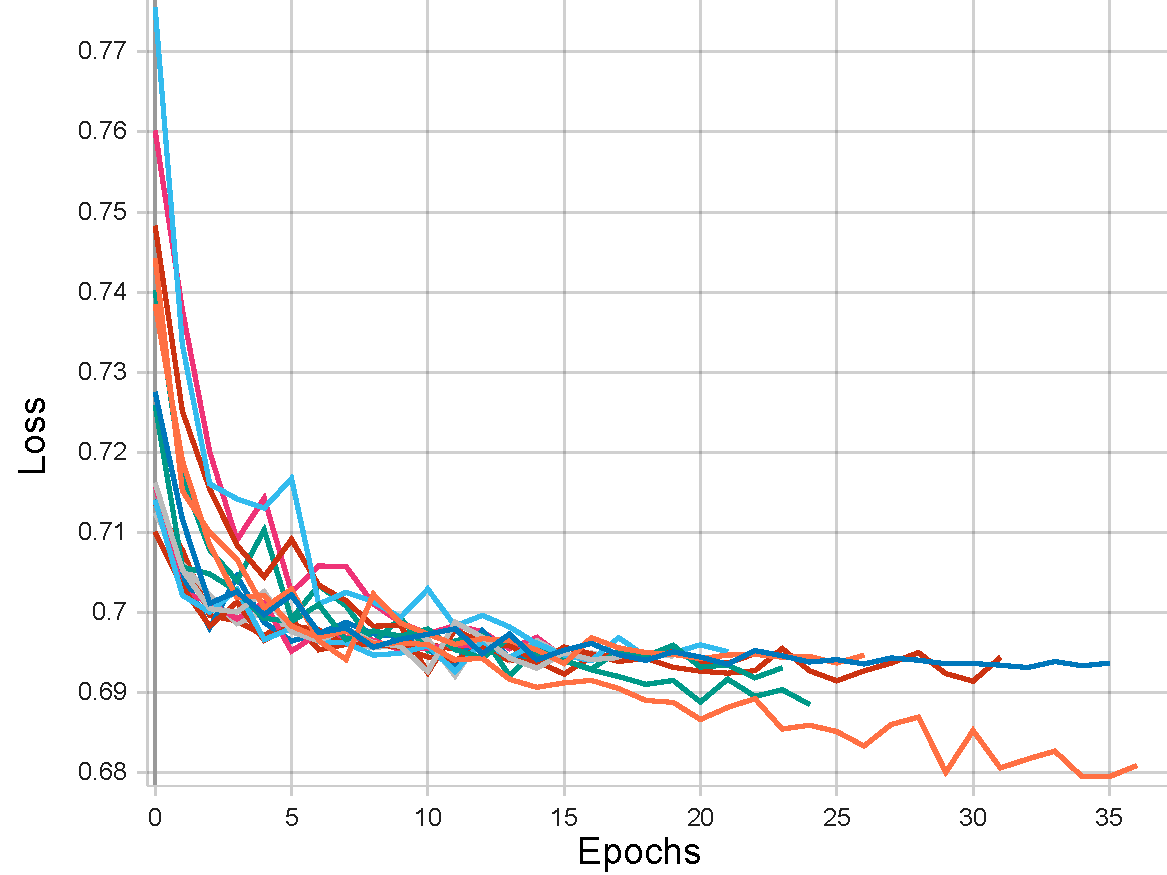
\includegraphics[width=0.575\columnwidth]{figures/results/final/week_loss_t.pdf}
    \caption[Training losses for Iteration 5 with one week of historic data]{Figure of all training losses with one week of historic data in Iteration 5}
    \label{fig:iteration5_week_train_loss}
\end{figure}
\FloatBarrier

\pagebreak
\textbf{Validation accuracies and losses}
\begin{figure}[ht]
    \centering
    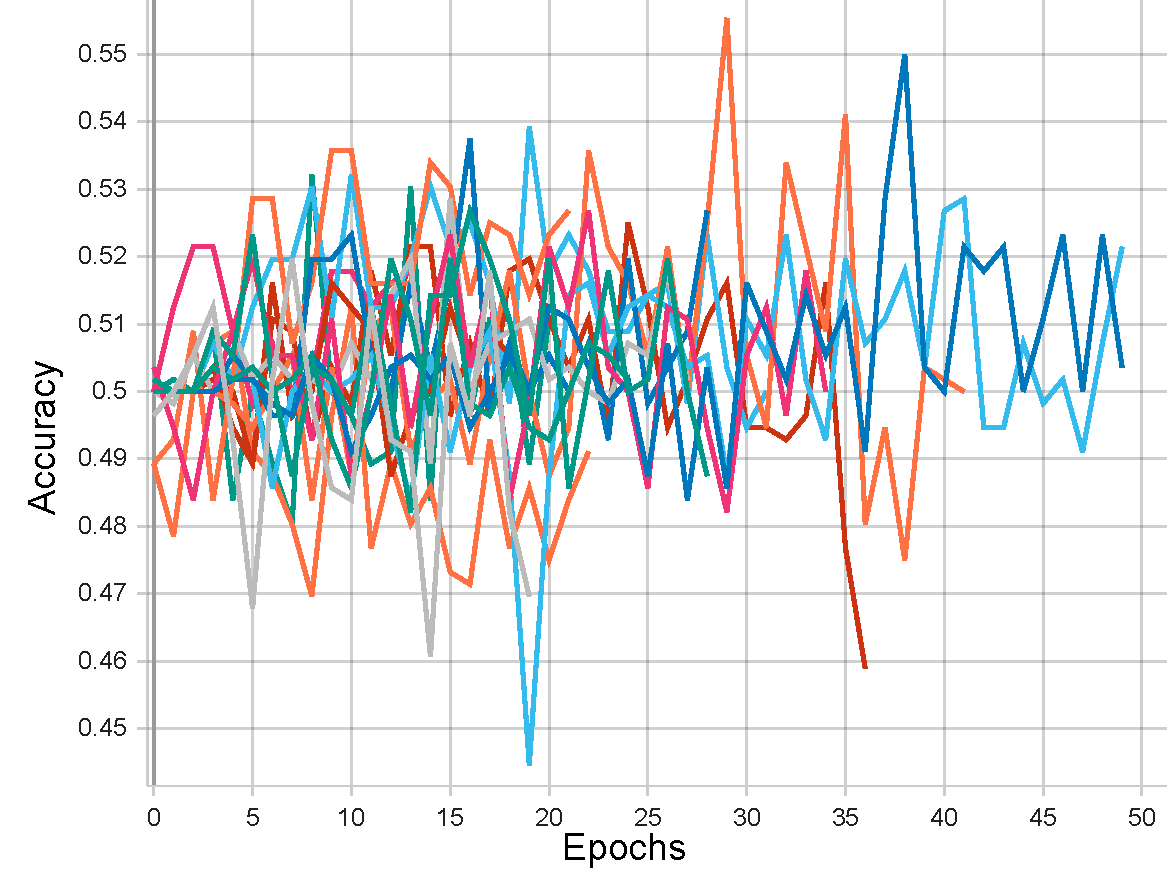
\includegraphics[width=0.575\columnwidth]{figures/results/final/week_acc.pdf}
    \caption[Validation accuracies for Iteration 5 with one week of historic data]{Figure of all validation accuracies with one week of historic data in Iteration 5}
    \label{fig:iteration5_week_accuracy}
\end{figure}
\FloatBarrier
\begin{figure}[ht]
    \centering
    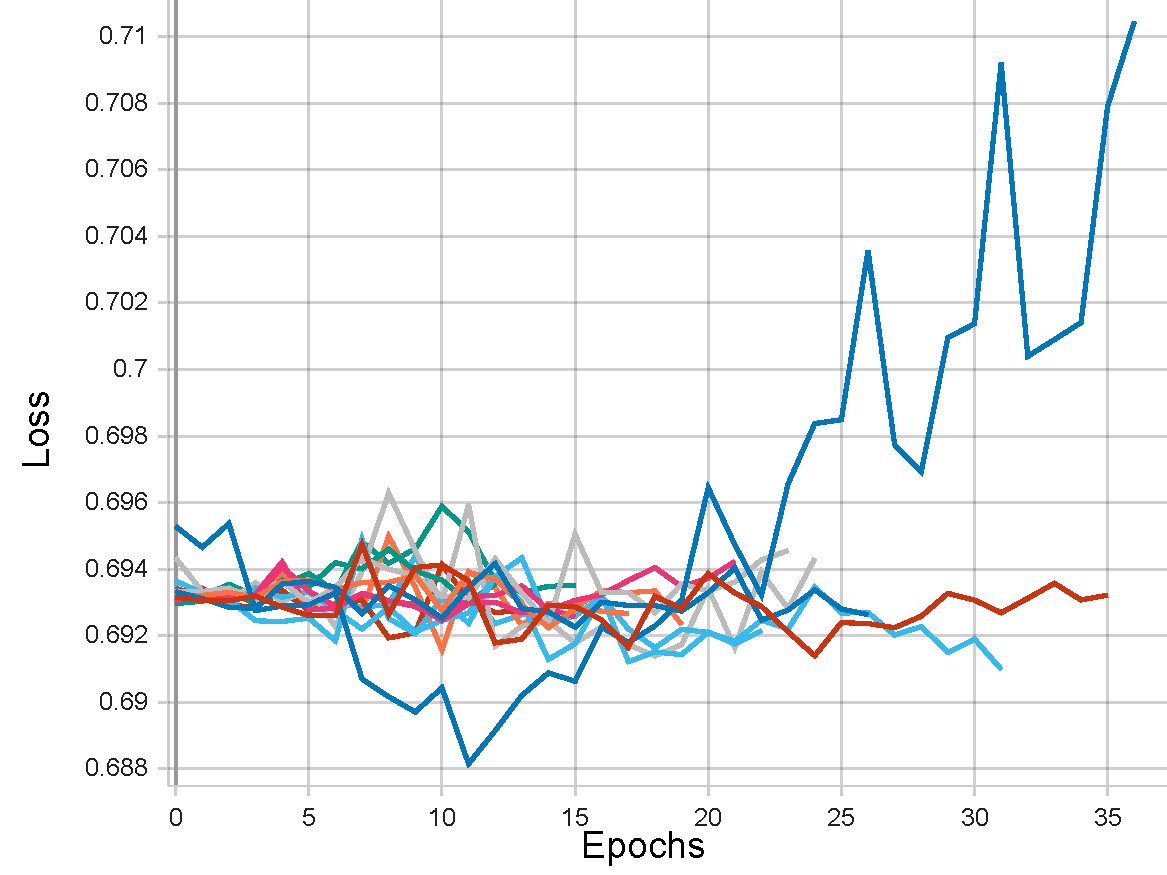
\includegraphics[width=0.575\columnwidth]{figures/results/final/week_loss.pdf}
    \caption[Validation losses for Iteration 5 with one week of historic data]{Figure of all validation losses with one week of historic data in Iteration 5}
    \label{fig:iteration5_week_loss}
\end{figure}
\FloatBarrier

The greatest validation accuracy for the model with a sequence length of one week was 55.54\% with the dataset using price and repurchase
agreements (repo) data.
While the chart above in \autoref{fig:iteration5_week_loss} may look erratic, the loss is actually minimal due to the scale as it only varies
between 0.688 and 0.713. This suggests there is little overfitting as it does not increase significantly.

\subsubsection{Two weeks of historic data accuracies and losses}
\textbf{Training accuracies and losses}
\begin{figure}[ht]
    \centering
    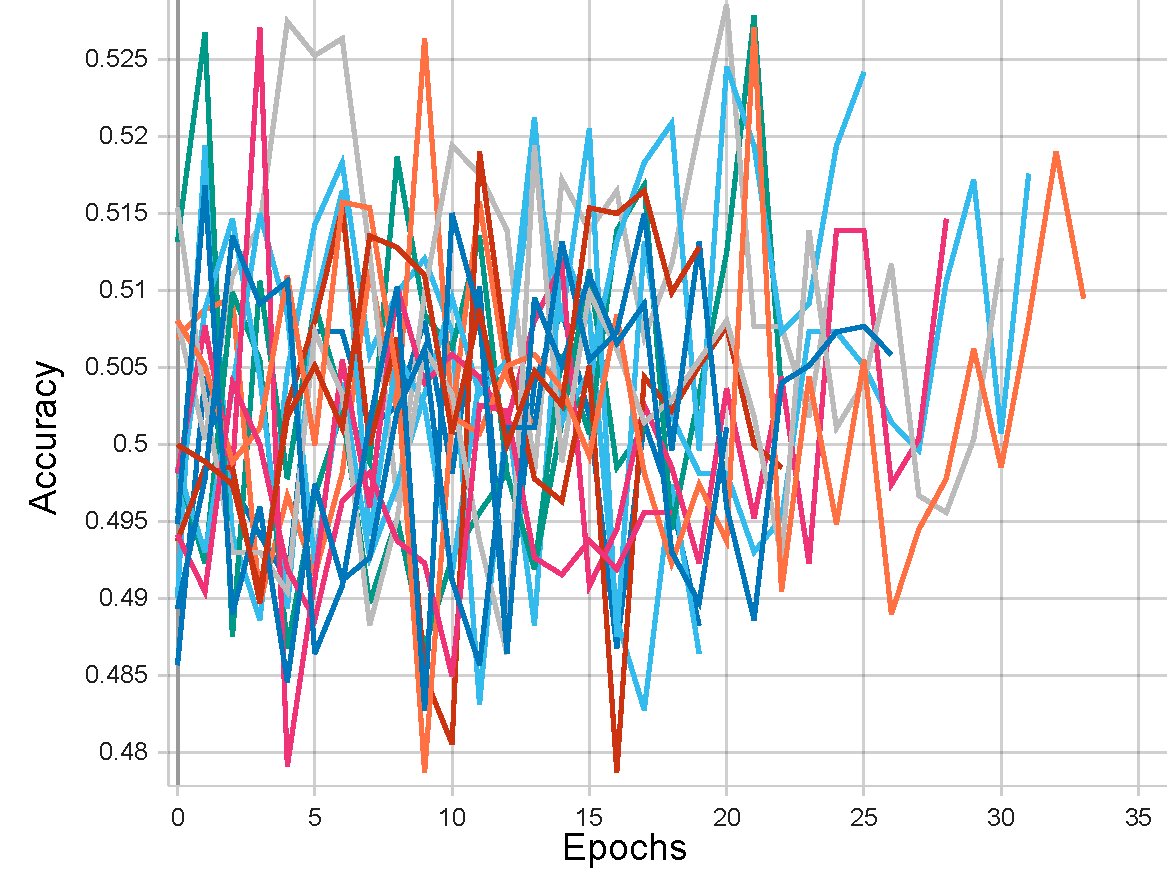
\includegraphics[width=0.575\columnwidth]{figures/results/final/two_weeks_acc_t.pdf}
    \caption[Training accuracies for Iteration 5 with two weeks of historic data]{Figure of all training accuracies with two weeks of historic data in Iteration 5}
    \label{fig:iteration5_two_weeks_train_accuracy}
\end{figure}
\FloatBarrier
\begin{figure}[ht]
    \centering
    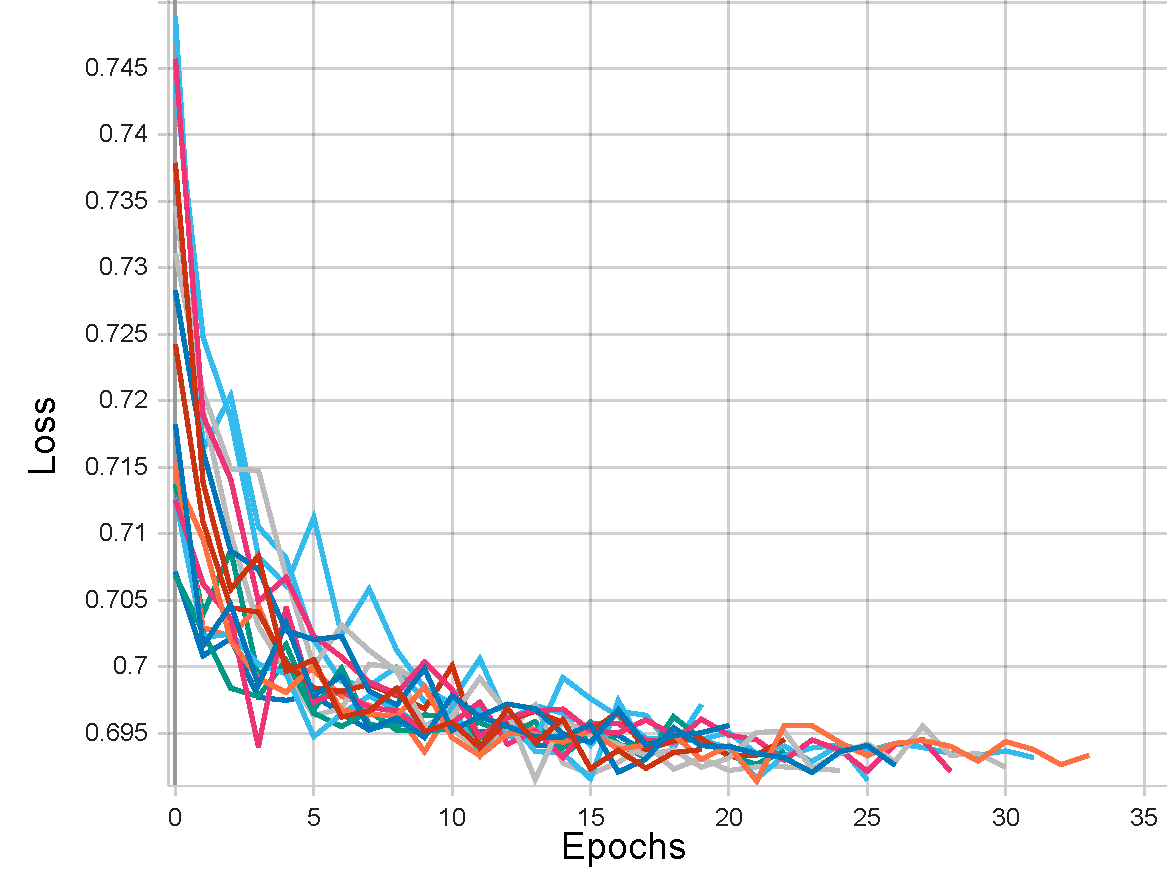
\includegraphics[width=0.575\columnwidth]{figures/results/final/two_weeks_loss_t.pdf}
    \caption[Training losses for Iteration 5 with two weeks of historic data]{Figure of all training losses with two weeks of historic data in Iteration 5}
    \label{fig:iteration5_two_weeks_train_loss}
\end{figure}
\FloatBarrier

\pagebreak
\textbf{Validation accuracies and losses}
\begin{figure}[ht]
    \centering
    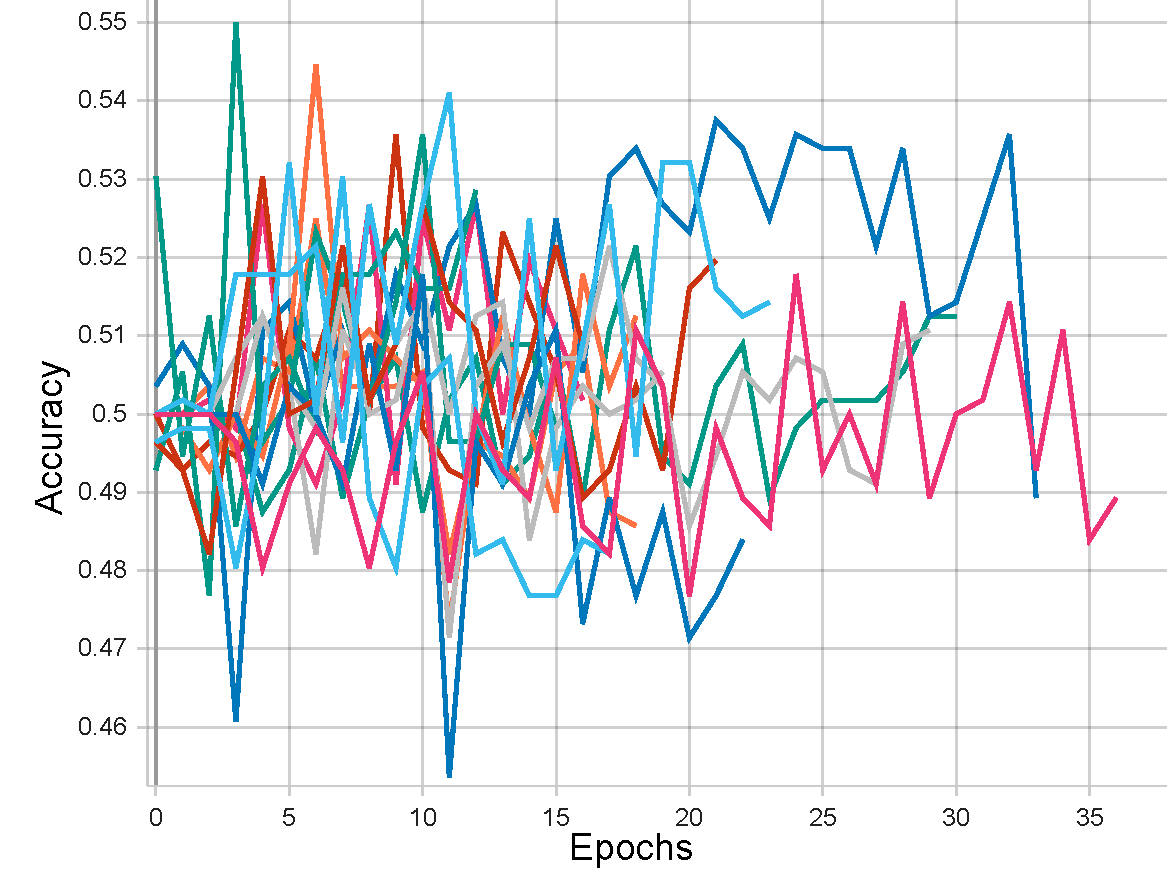
\includegraphics[width=0.575\columnwidth]{figures/results/final/two_weeks_acc.pdf}
    \caption[Validation accuracies for Iteration 5 with two weeks of historic data]{Figure of all validation accuracies with two weeks of historic data in Iteration 5}
    \label{fig:iteration5_two_weeks_accuracy}
\end{figure}
\FloatBarrier
\begin{figure}[ht]
    \centering
    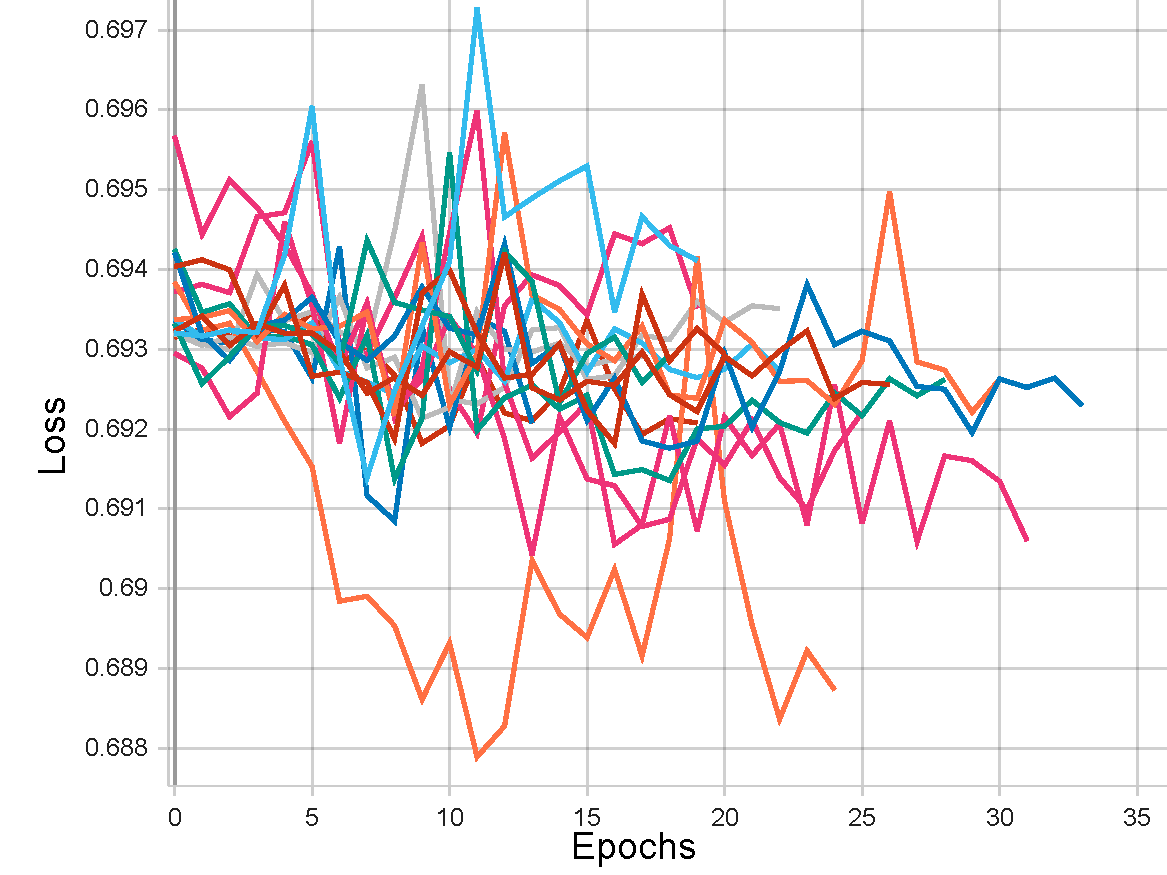
\includegraphics[width=0.575\columnwidth]{figures/results/final/two_weeks_loss.pdf}
    \caption[Validation losses for Iteration 5 with two weeks of historic data]{Figure of all validation losses with two weeks of historic data in Iteration 5}
    \label{fig:iteration5_two_weeks_loss}
\end{figure}
\FloatBarrier

The greatest validation accuracy for the model with a sequence length of two weeks was 55.18\% with the dataset using price and repurchase
agreements (repo) data.
While the chart above in \autoref{fig:iteration5_two_weeks_loss} may look erratic, the loss is actually minimal due to the scale as it only varies
between 0.688 and 0.697. This suggests there is little overfitting as it does not increase significantly.

\subsubsection{One month of historic data accuracies and losses}
\textbf{Training accuracies and losses}
\begin{figure}[ht]
    \centering
    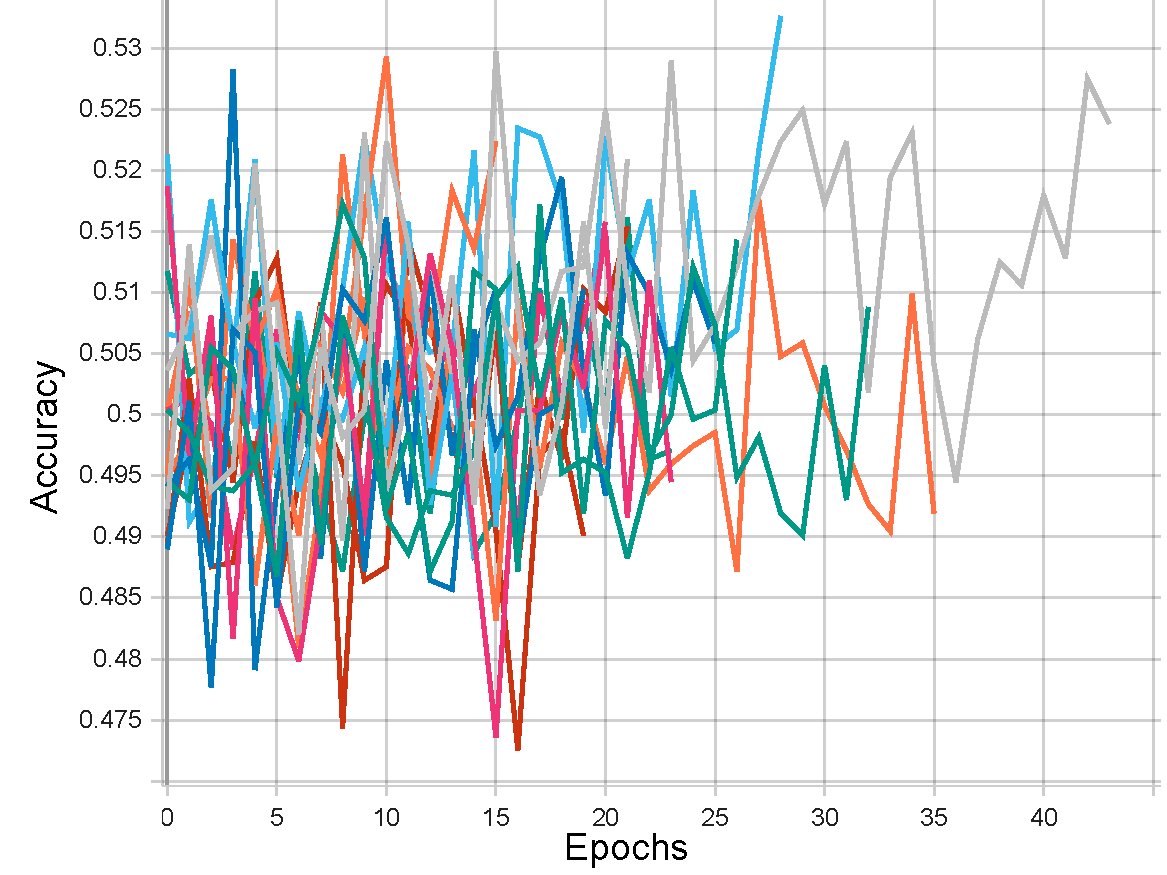
\includegraphics[width=0.575\columnwidth]{figures/results/final/month_acc_t.pdf}
    \caption[Training accuracies for Iteration 5 with one month of historic data]{Figure of all training accuracies with one month of historic data in Iteration 5}
    \label{fig:iteration5_month_train_accuracy}
\end{figure}
\FloatBarrier
\begin{figure}[ht]
    \centering
    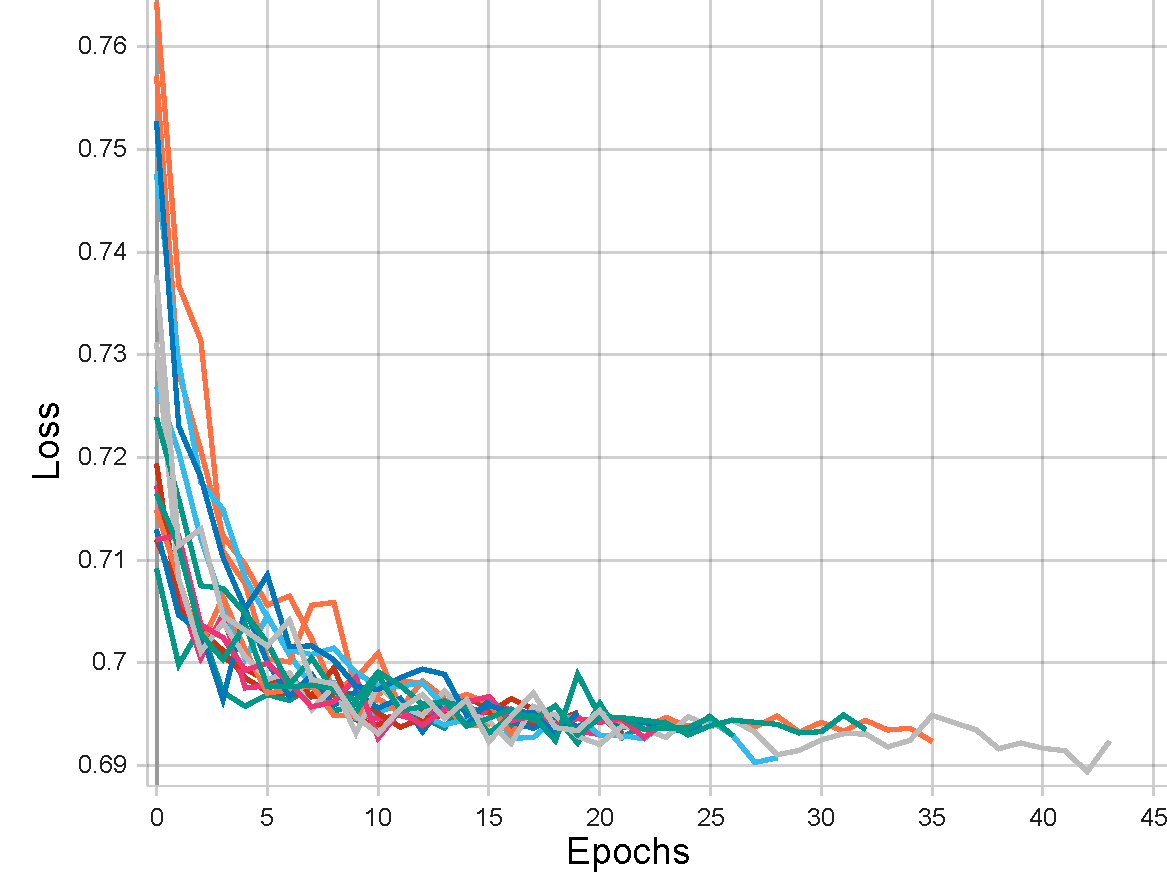
\includegraphics[width=0.575\columnwidth]{figures/results/final/month_loss_t.pdf}
    \caption[Training losses for Iteration 5 with one month of historic data]{Figure of all training losses with one month of historic data in Iteration 5}
    \label{fig:iteration5_month_train_loss}
\end{figure}
\FloatBarrier

\pagebreak
\textbf{Validation accuracies and losses}
\begin{figure}[ht]
    \centering
    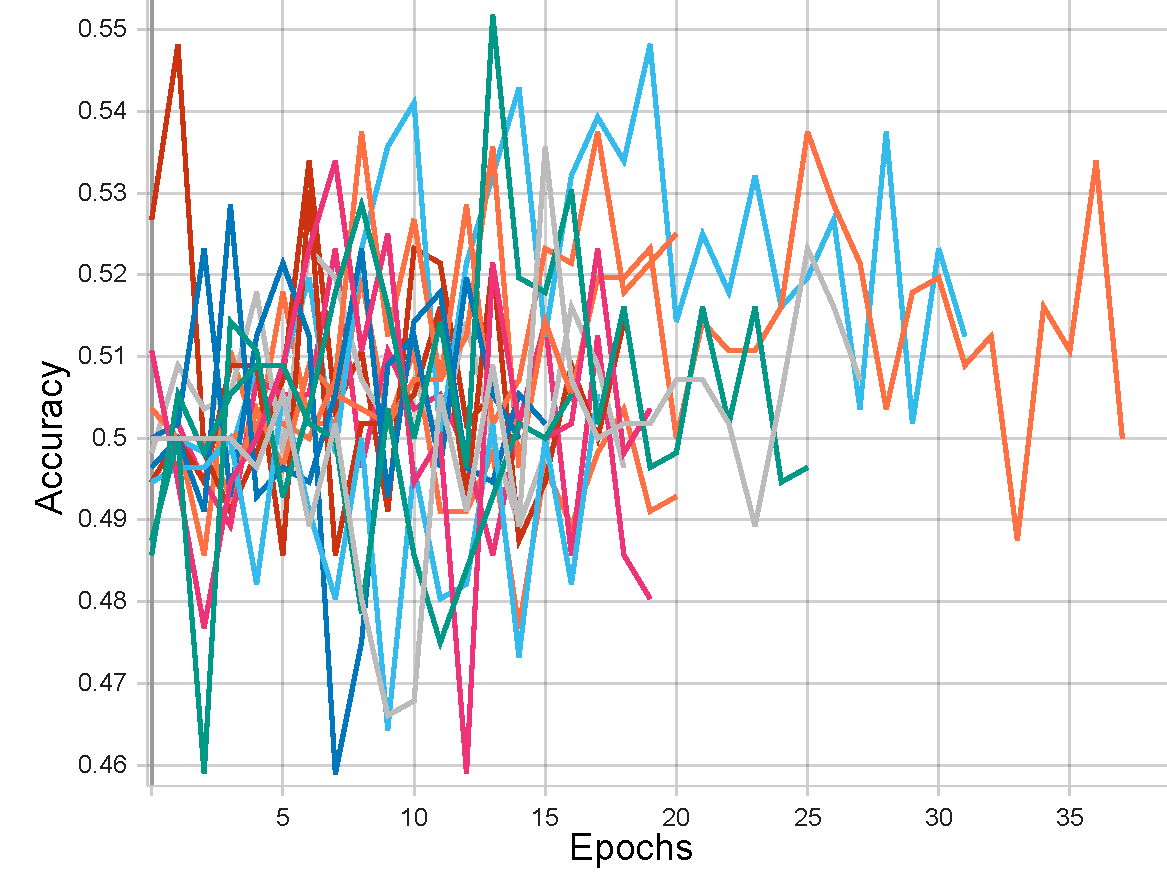
\includegraphics[width=0.575\columnwidth]{figures/results/final/month_acc.pdf}
    \caption[Validation accuracies for Iteration 5 with one month of historic data]{Figure of all validation accuracies with one month of historic data in Iteration 5}
    \label{fig:iteration5_month_accuracy}
\end{figure}
\FloatBarrier
\begin{figure}[ht]
    \centering
    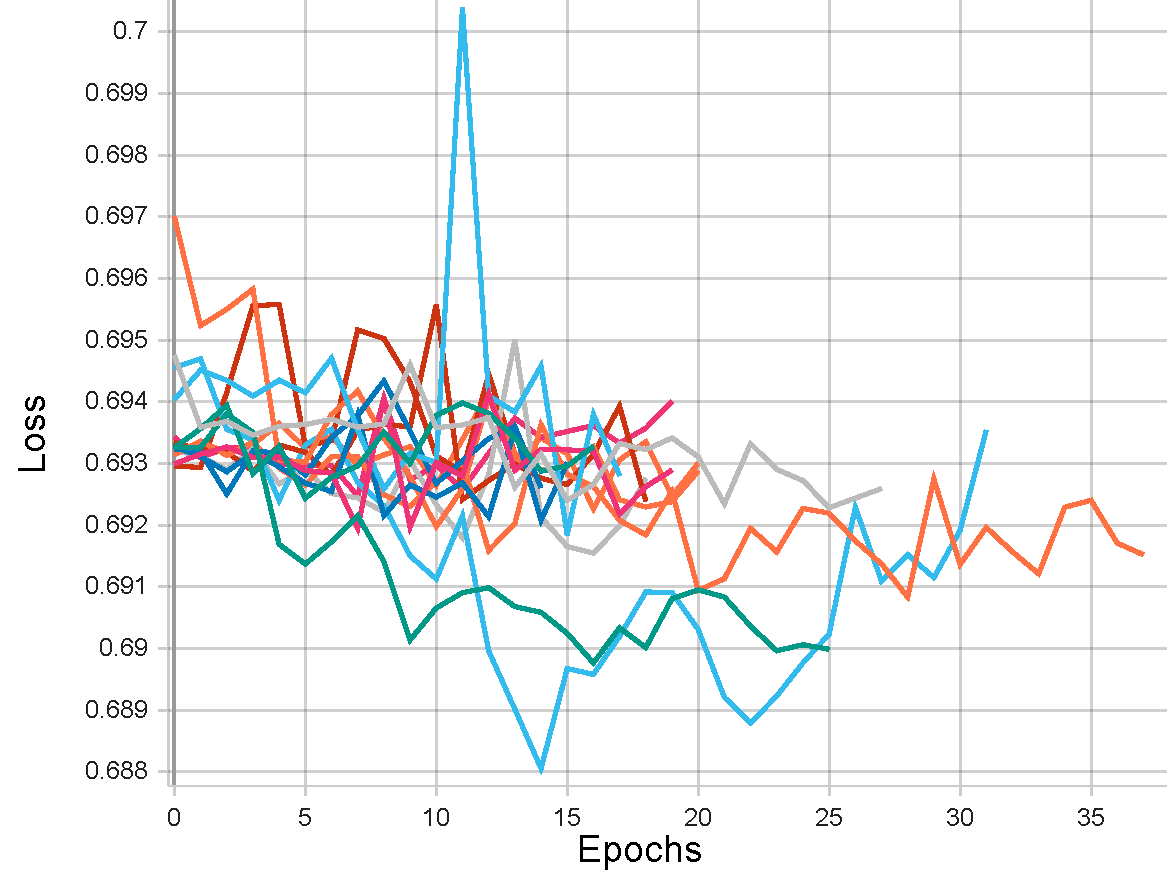
\includegraphics[width=0.575\columnwidth]{figures/results/final/month_loss.pdf}
    \caption[Validation losses for Iteration 5 with one month of historic data]{Figure of all validation losses with one month of historic data in Iteration 5}
    \label{fig:iteration5_month_loss}
\end{figure}
\FloatBarrier

The greatest validation accuracy for the model with a sequence length of two weeks was 57.50\% with the dataset using price
and treasury yields data.
While the chart above in \autoref{fig:iteration5_month_loss} may look erratic, the loss is actually minimal due to the scale as it only varies
between 0.687 and 0.696. This suggests there is little overfitting as it does not increase significantly.

\pagebreak
\subsubsection{Two months of historic data accuracies and losses}
\textbf{Training accuracies and losses}
\begin{figure}[ht]
    \centering
    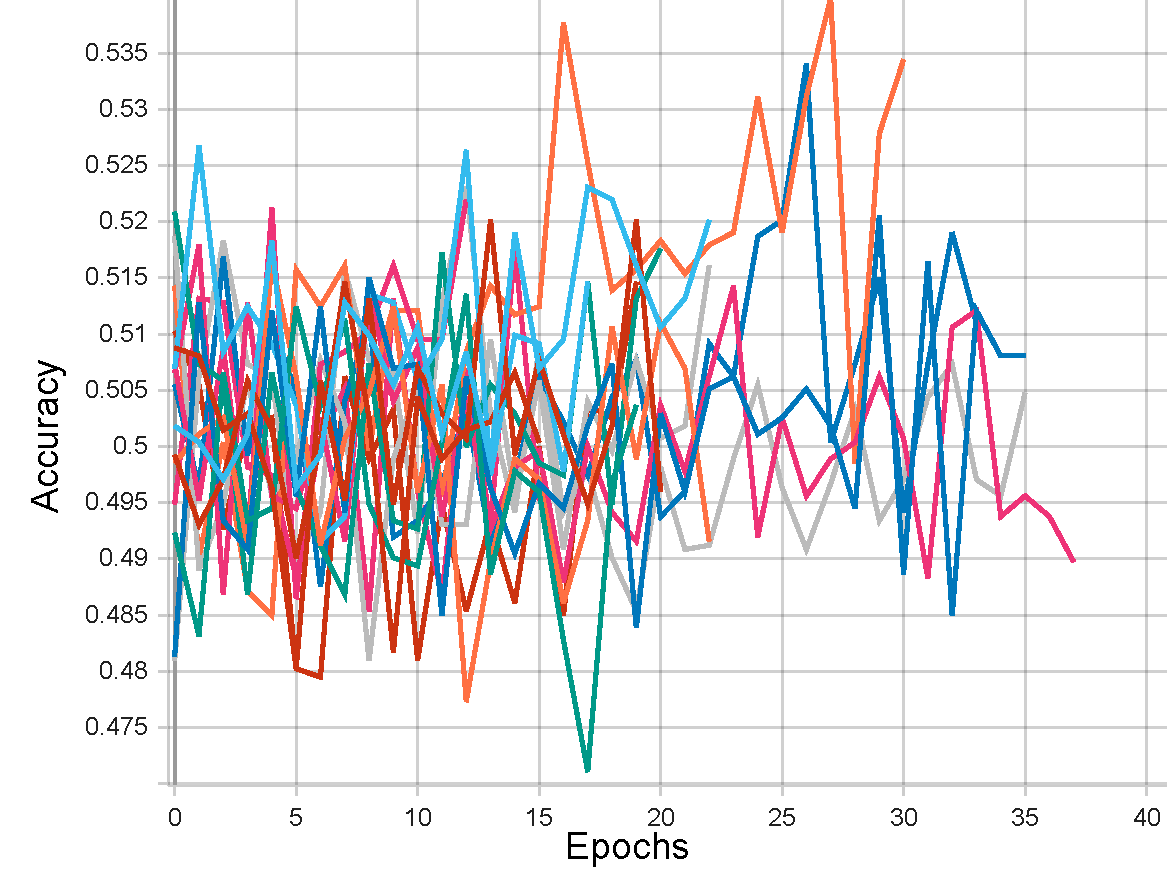
\includegraphics[width=0.575\columnwidth]{figures/results/final/two_months_acc_t.pdf}
    \caption[Training accuracies for Iteration 5 with two months of historic data]{Figure of all training accuracies with two months of historic data in Iteration 5}
    \label{fig:iteration5_two_months_train_accuracy}
\end{figure}
\FloatBarrier
\begin{figure}[ht]
    \centering
    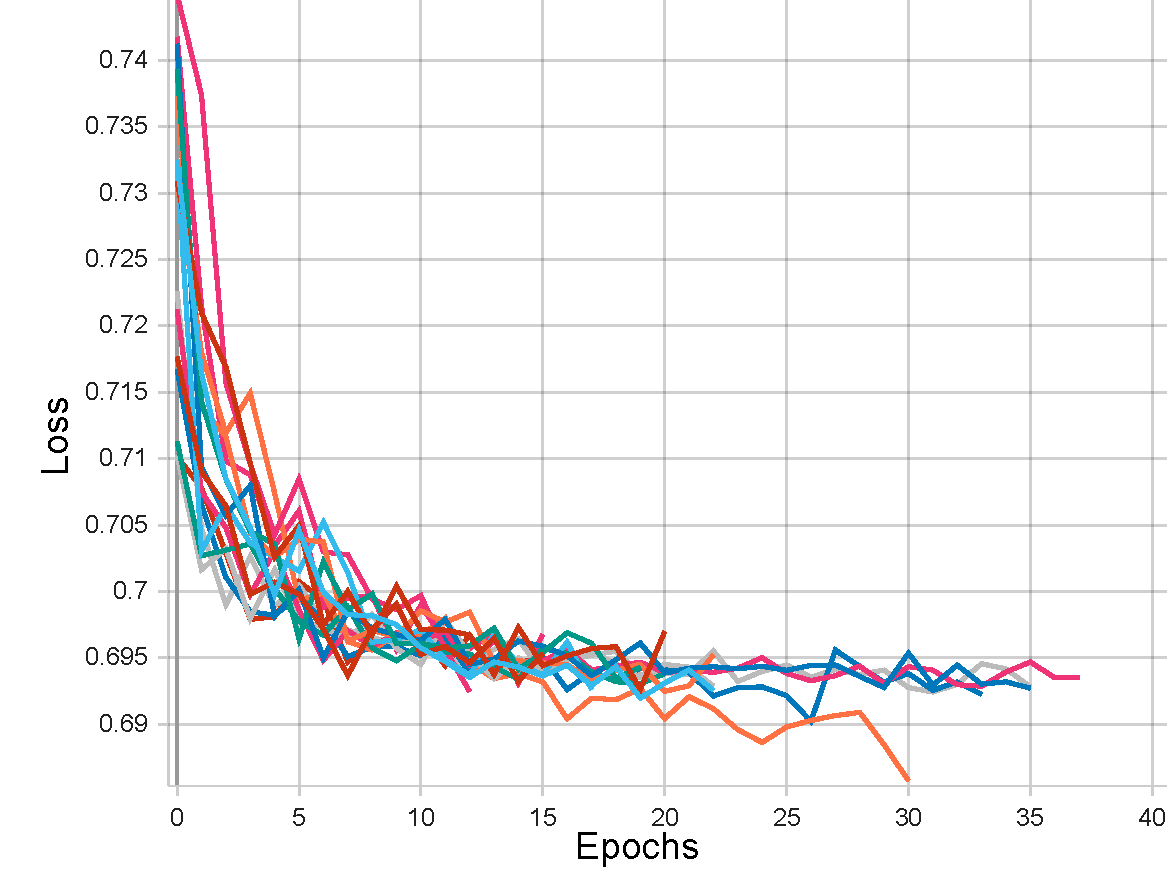
\includegraphics[width=0.575\columnwidth]{figures/results/final/two_months_loss_t.pdf}
    \caption[Training losses for Iteration 5 with two months of historic data]{Figure of all training losses with two months of historic data in Iteration 5}
    \label{fig:iteration5_two_months_train_loss}
\end{figure}
\FloatBarrier

\pagebreak
\textbf{Validation accuracies and losses}
\begin{figure}[ht]
    \centering
    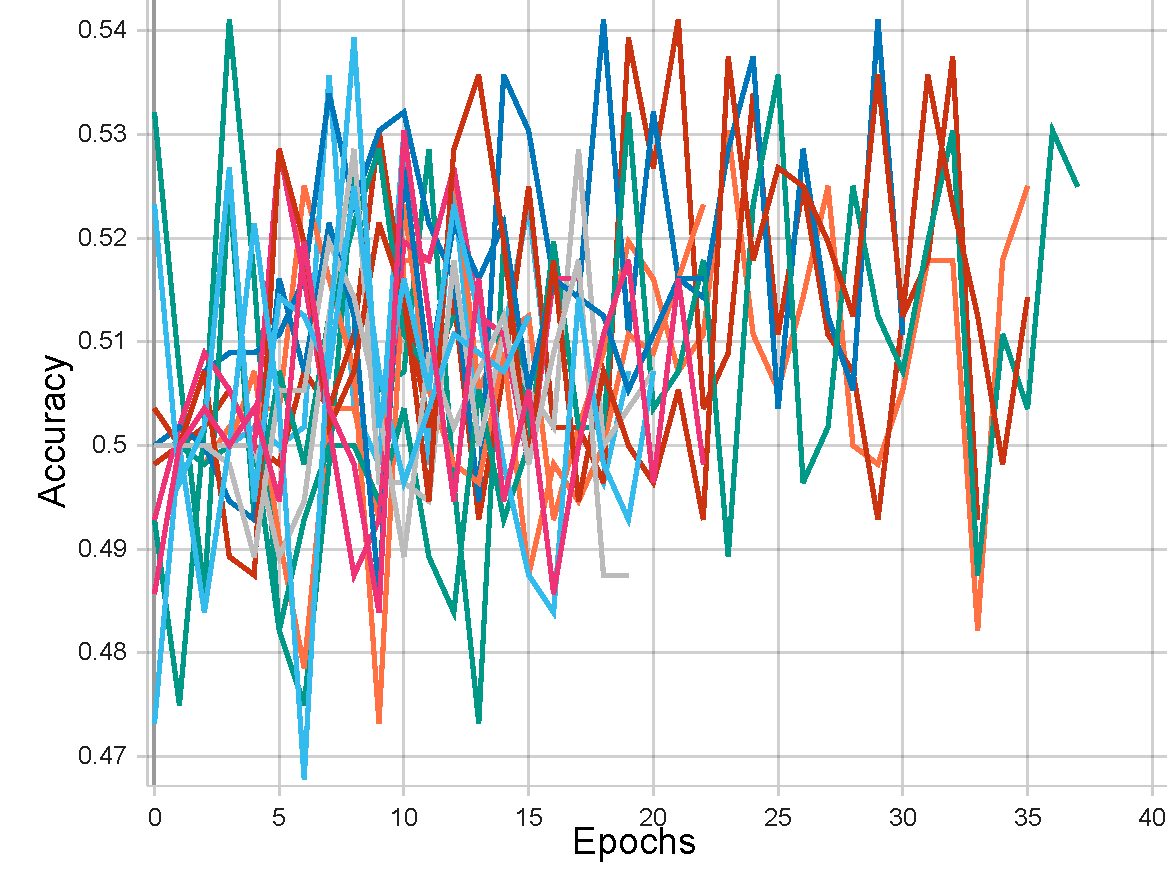
\includegraphics[width=0.575\columnwidth]{figures/results/final/two_months_acc.pdf}
    \caption[Validation accuracies for Iteration 5 with two months of historic data]{Figure of all validation accuracies with two months of historic data in Iteration 5}
    \label{fig:iteration5_two_months_accuracy}
\end{figure}
\FloatBarrier
\begin{figure}[ht]
    \centering
    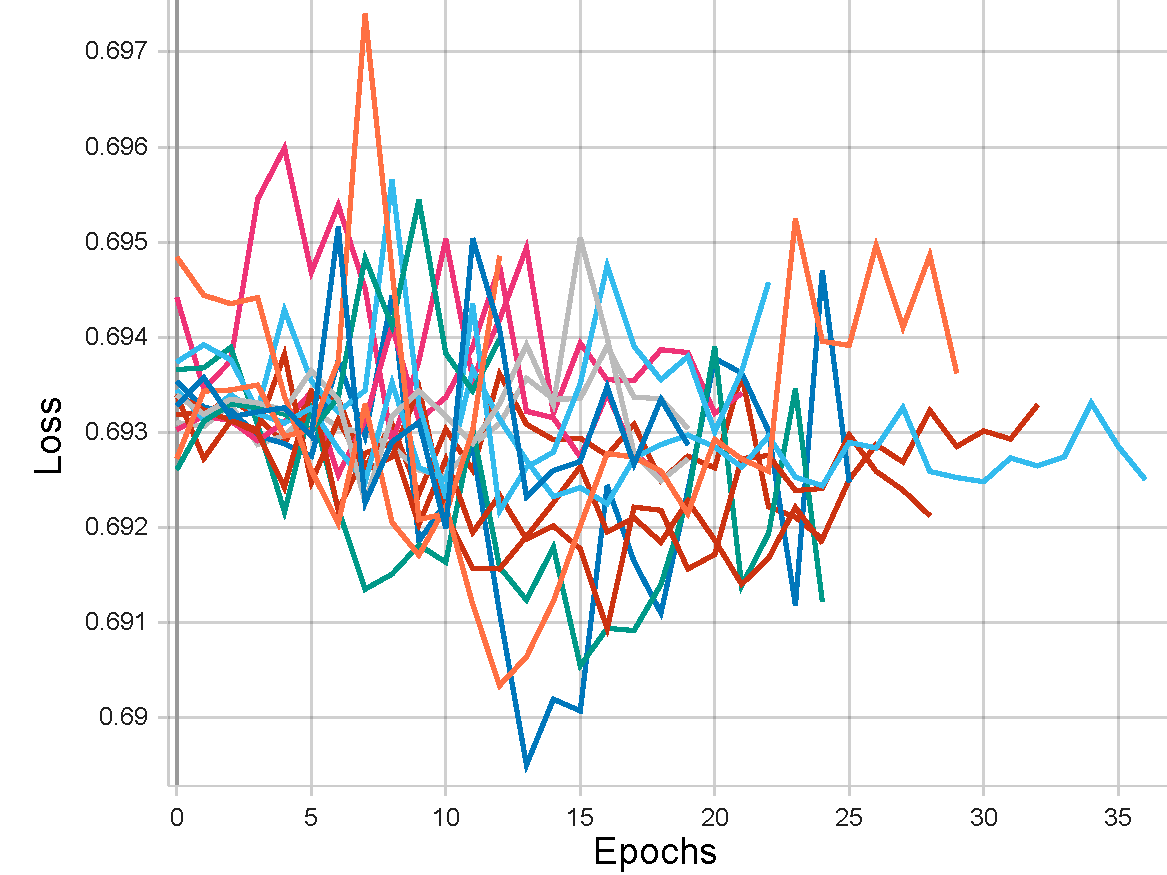
\includegraphics[width=0.575\columnwidth]{figures/results/final/two_months_loss.pdf}
    \caption[Validation losses for Iteration 5 with two months of historic data]{Figure of all validation losses with two months of historic data in Iteration 5}
    \label{fig:iteration5_two_months_loss}
\end{figure}
\FloatBarrier

The greatest validation accuracy for the model with a sequence length of two weeks was 54.11\% with the dataset using the extended price
changes dataset, the price and volatility data, or the price and treasury yields data.
While the chart above in \autoref{fig:iteration5_two_months_loss} may look erratic, the loss is actually minimal due to the scale as it only varies
between 0.689 and 0.703. This suggests there is little overfitting as it does not increase significantly.

\subsubsection{One quarter of historic data accuracies and losses}
\textbf{Training accuracies and losses}
\begin{figure}[ht]
    \centering
    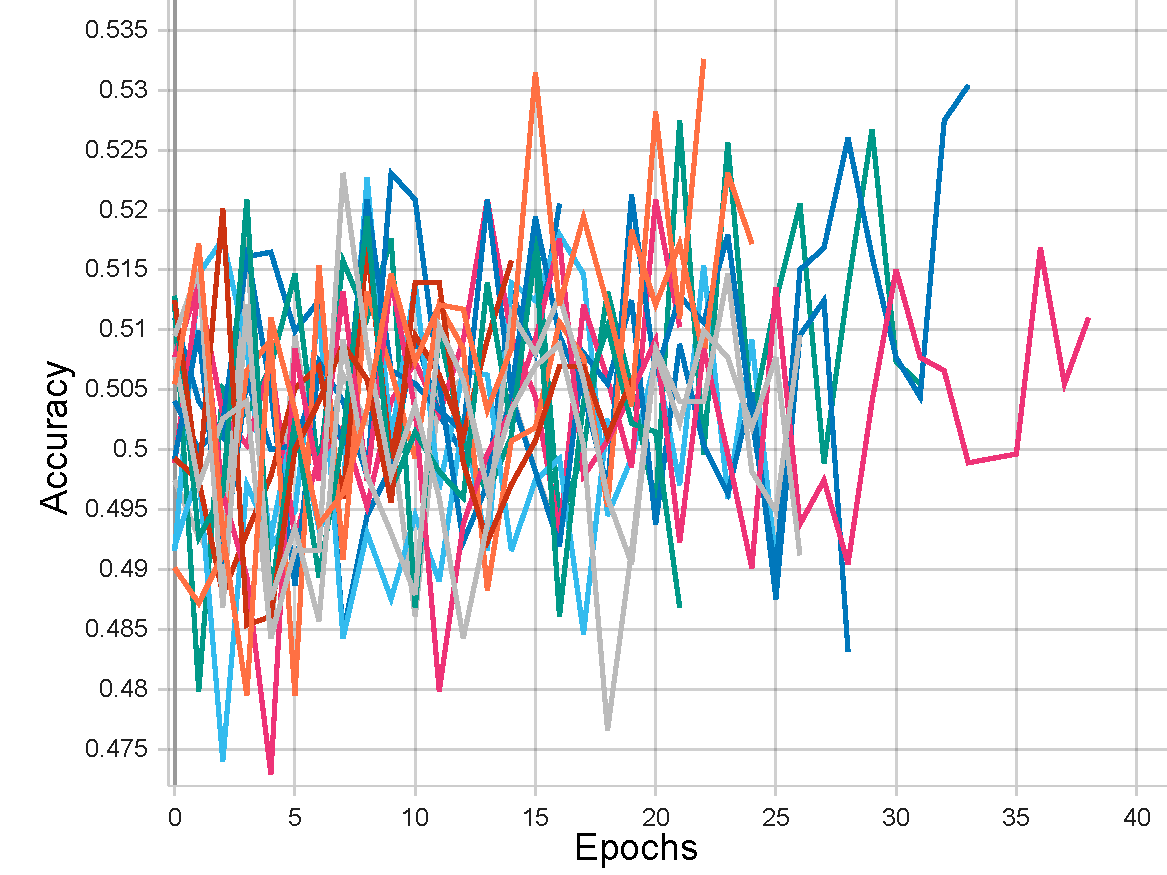
\includegraphics[width=0.575\columnwidth]{figures/results/final/quarter_acc_t.pdf}
    \caption[Training accuracies for Iteration 5 with one quarter of historic data]{Figure of all training accuracies with one quarter of historic data in Iteration 5}
    \label{fig:iteration5_quarter_train_accuracy}
\end{figure}
\FloatBarrier
\begin{figure}[ht]
    \centering
    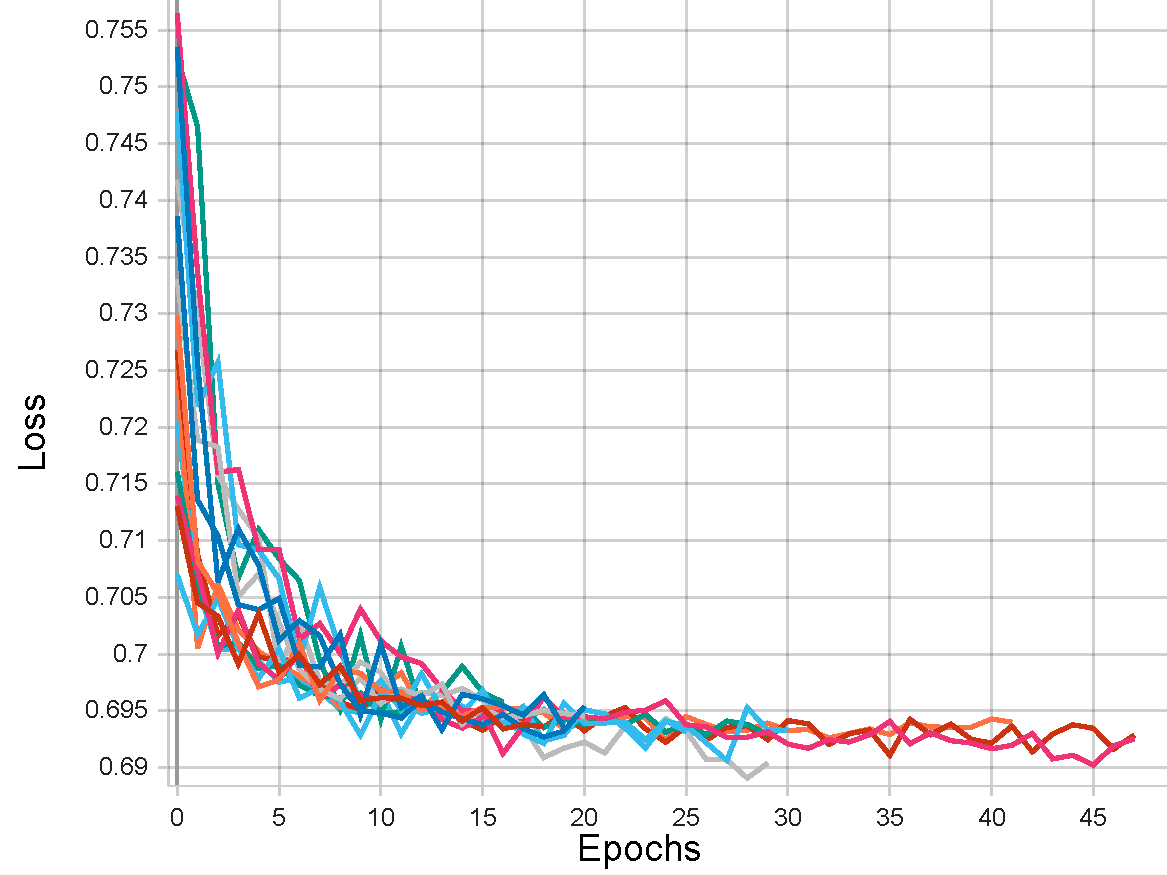
\includegraphics[width=0.575\columnwidth]{figures/results/final/quarter_loss_t.pdf}
    \caption[Training losses for Iteration 5 with one quarter of historic data]{Figure of all training losses with one quarter of historic data in Iteration 5}
    \label{fig:iteration5_quarter_train_loss}
\end{figure}
\FloatBarrier

\pagebreak
\textbf{Validation accuracies and losses}
\begin{figure}[ht]
    \centering
    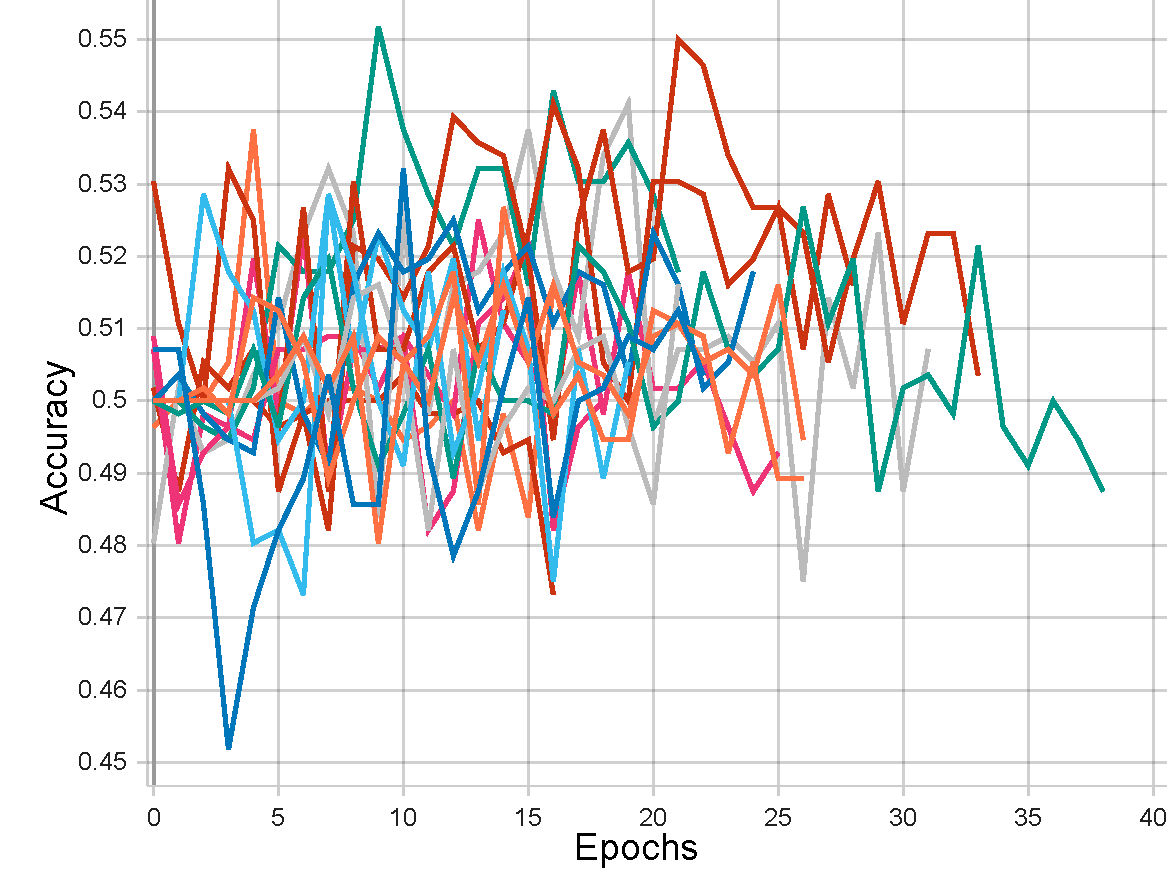
\includegraphics[width=0.575\columnwidth]{figures/results/final/quarter_acc.pdf}
    \caption[Validation accuracies for Iteration 5 with one quarter of historic data]{Figure of all validation accuracies with one quarter of historic data in Iteration 5}
    \label{fig:iteration5_quarter_accuracy}
\end{figure}
\FloatBarrier
\begin{figure}[ht]
    \centering
    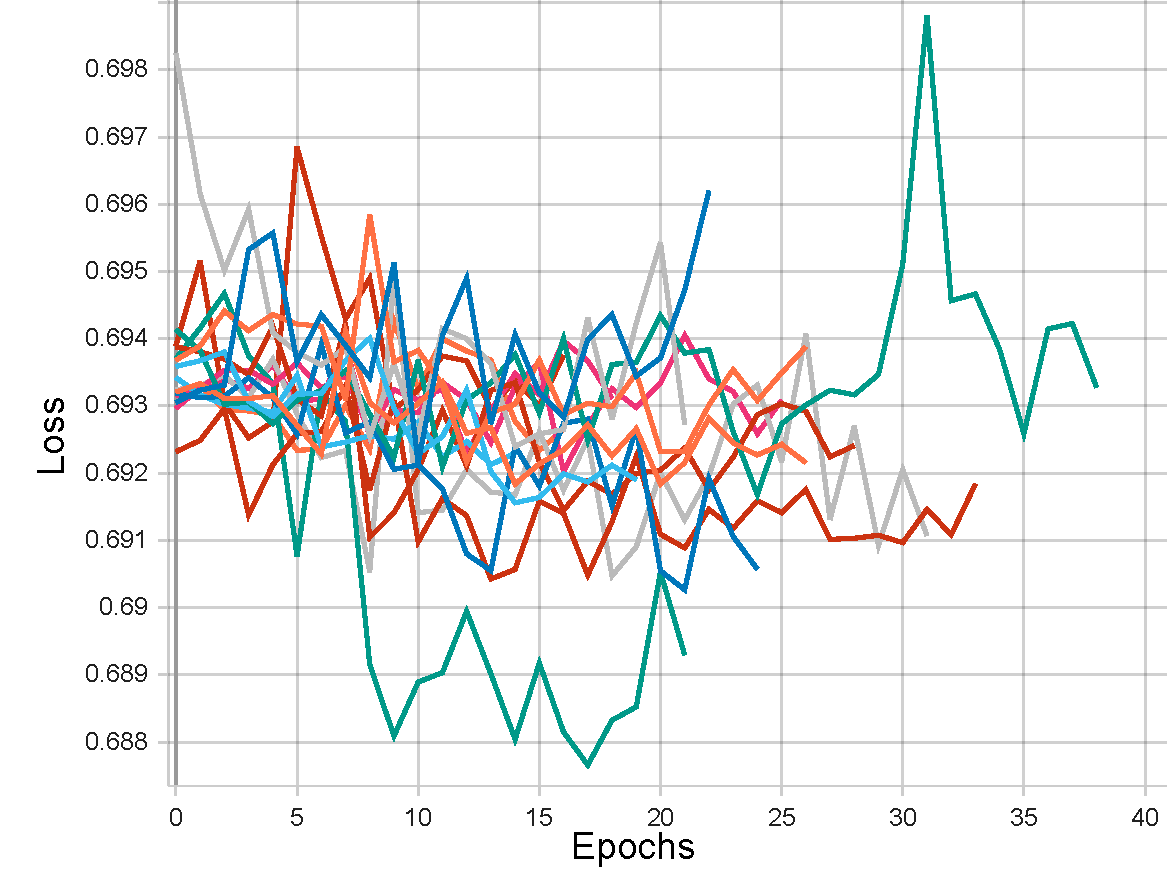
\includegraphics[width=0.575\columnwidth]{figures/results/final/quarter_loss.pdf}
    \caption[Validation losses for Iteration 5 with one quarter of historic data]{Figure of all validation losses with one quarter of historic data in Iteration 5}
    \label{fig:iteration5_quarter_loss}
\end{figure}
\FloatBarrier

The greatest validation accuracy for the model with a sequence length of two weeks was 55.18\% with the dataset of the price and treasury yields data.
While the chart above in \autoref{fig:iteration5_quarter_loss} may look erratic, the loss is actually minimal due to the scale as it only varies
between 0.687 and 0.699. This suggests there is little overfitting as it does not increase significantly.

\subsection{Comparisions of models in iteration 5}\label{ssec:iteration5_best_val_acc}
The table below in \autoref{fig:final_val_accuracy} shows the accuracies of each combination of input features and length of historic data.
\begin{figure}[ht]
    \centering
    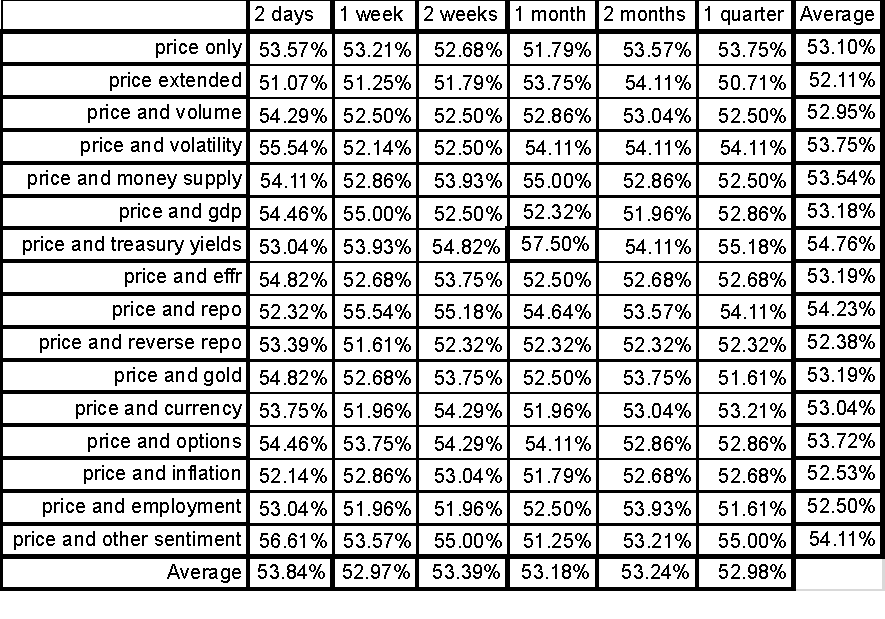
\includegraphics[width=0.95\columnwidth]{figures/results/final/final_val_accuracy.pdf}
    \caption[Best validation accuracies for Iteration 5]{Figure of all validation accuracies of each combination of input features and sequence length in Iteration 5}
    \label{fig:final_val_accuracy}
\end{figure}
\FloatBarrier

The results show the model of the stock market index price combined with treasury yield data and 
a sequence length of 1 month (21 days) of historic data, has the best accuracy with a value of
57.50\%.

However, there is additional data that can be inferred from the results. On average, the model with a sequence
length of two days performs the best with a validation accuracy of 53.84\%. This suggests that the stock markets may react
strongest to short term changes. The models' accuracies slightly decrease for the one-week sequence length, and fluctuate
slightly across other sequence lengths but never increase over the model with a sequence length of two days.

On average, the model utilising price and treasury yields data, have the highest average validation accuracy of 54.76\%. This
shows that treasury yields data can be an important factor to stock market returns.

In order to better visualise how different features affect the model, each combination of input features was compared against the `price only' dataset for each sequence length.
The results of these comparisions can be shown in the table below in \autoref{fig:val_accuracy_comparison}.

\begin{figure}[ht]
    \centering
    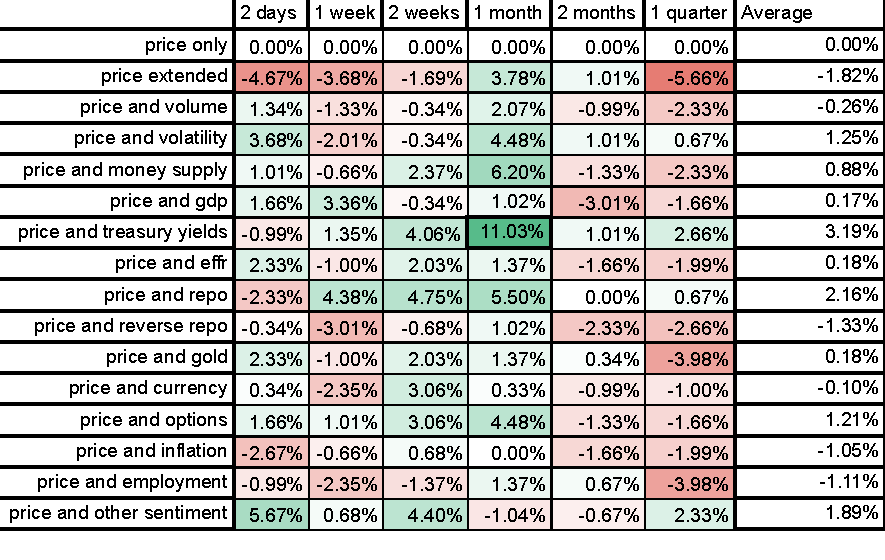
\includegraphics[width=0.95\columnwidth]{figures/results/final/val_accuracy_comparison.pdf}
    \caption[Best validation accuracies for Iteration 5]{Figure of all validation accuracies of each combination of input features and sequence length in Iteration 5}
    \label{fig:val_accuracy_comparison}
\end{figure}
\FloatBarrier

The model with a sequence length of two days does not see many significant improvements with most combinations of input features.
For sequence lengths, many factors can have a positive impact to the models, the results above show that volume, volatility,
M1 money supply, GDP, Effective Federal Funds Rate (EFFR), gold prices, currency exchange rates, put-to-call ratio (options), and other
sentiment data. Whereas for sequence lengths of one month, there is some overlap of important factors that affect the accuracy of the models.
The factors that impact one month sequence lengths are the extended price dataset, as well as volume, volatility, M1 money supply, GDP, 
treasury yields, EFFR, Repurchase Agreements (Repo) utilisation and rates, Reverse Repo utilisation and rates, gold prices, currency exchange rates,
and put-to-call ratio (options) data.

\subsection{Evaluation of iteration 5}

